% Capitolul 4: Modele SARIMA pentru Serii de Timp Sezoniere
% Prezentare academică de calitate Harvard
% Program de licență, Academia de Studii Economice din București

\documentclass[9pt, aspectratio=169, t]{beamer}

% Asigură încadrarea conținutului pe diapozitive
\setbeamersize{text margin left=8mm, text margin right=8mm}

%=============================================================================
% CONFIGURARE TEMĂ ȘI STIL
%=============================================================================
\usetheme{default}
% Utilizăm tema implicită pentru control curat al antetului/subsolului

% Paletă de Culori (potrivită cu PDF-ul Redispatch)
\definecolor{MainBlue}{RGB}{26, 58, 110}
\definecolor{AccentBlue}{RGB}{26, 58, 110}
\definecolor{IDAred}{RGB}{205, 0, 0}
\definecolor{DarkGray}{RGB}{51, 51, 51}
\definecolor{MediumGray}{RGB}{128, 128, 128}
\definecolor{LightGray}{RGB}{248, 248, 248}
\definecolor{VeryLightGray}{RGB}{235, 235, 235}
\definecolor{KeynoteGray}{RGB}{218, 218, 218}
\definecolor{SectionGray}{RGB}{120, 120, 120}
\definecolor{FooterGray}{RGB}{100, 100, 100}
\definecolor{Crimson}{RGB}{220, 53, 69}
\definecolor{Forest}{RGB}{46, 125, 50}
\definecolor{Amber}{RGB}{181, 133, 63}
\definecolor{Orange}{RGB}{230, 126, 34}
\definecolor{Purple}{RGB}{142, 68, 173}

% Fundal gradient (gradient Keynote exact 315°: alb la RGB 218,218,218)
\setbeamertemplate{background}{%
    \begin{tikzpicture}[remember picture, overlay]
        \shade[shading=axis, shading angle=315,
        top color=white, bottom color=KeynoteGray]
        (current page.south west) rectangle (current page.north east);
    \end{tikzpicture}%
}
% Culoare solidă de rezervă pentru compatibilitate
\setbeamercolor{background canvas}{bg=}

\setbeamercolor{palette primary}{bg=MainBlue, fg=white}
\setbeamercolor{palette secondary}{bg=MainBlue!85, fg=white}
\setbeamercolor{palette tertiary}{bg=MainBlue!70, fg=white}
\setbeamercolor{structure}{fg=MainBlue}
\setbeamercolor{title}{fg=IDAred}
\setbeamercolor{frametitle}{fg=IDAred, bg=}
\setbeamercolor{block title}{bg=MainBlue, fg=white}
\setbeamercolor{block body}{bg=VeryLightGray, fg=DarkGray}
\setbeamercolor{block title alerted}{bg=Crimson, fg=white}
\setbeamercolor{block body alerted}{bg=Crimson!8, fg=DarkGray}
\setbeamercolor{block title example}{bg=Forest, fg=white}
\setbeamercolor{block body example}{bg=Forest!8, fg=DarkGray}
\setbeamercolor{item}{fg=MainBlue}

% Culori subsol (suprascriu albastrul temei Madrid)
\setbeamercolor{author in head/foot}{fg=FooterGray, bg=}
\setbeamercolor{title in head/foot}{fg=FooterGray, bg=}
\setbeamercolor{date in head/foot}{fg=FooterGray, bg=}
\setbeamercolor{section in head/foot}{fg=FooterGray, bg=}
\setbeamercolor{subsection in head/foot}{fg=FooterGray, bg=}

% Stiluri marcatori (se aplică peste tot inclusiv în blocuri)
\setbeamertemplate{itemize item}{\color{MainBlue}$\boxdot$}
\setbeamertemplate{itemize subitem}{\color{MainBlue}$\blacktriangleright$}
\setbeamertemplate{itemize subsubitem}{\color{MainBlue}\tiny$\bullet$}
\setbeamertemplate{itemize/enumerate body begin}{\normalsize}
\setbeamertemplate{itemize/enumerate subbody begin}{\normalsize}

% Item spacing - compact style
\setlength{\leftmargini}{10pt}       % Level 1: minimal indent
\setlength{\leftmarginii}{10pt}      % Level 2: minimal additional indent
% Compact list spacing (zero extra space before/after lists in blocks)
\makeatletter
\def\@listi{\leftmargin\leftmargini \topsep 0pt \parsep 0pt \itemsep 0pt}
\def\@listii{\leftmargin\leftmarginii \topsep 0pt \parsep 0pt \itemsep 0pt}
\makeatother

\setbeamertemplate{navigation symbols}{}

%=============================================================================
% ANTET PERSONALIZAT
%=============================================================================
\setbeamertemplate{headline}{%
    \vskip10pt%
    \hbox to \paperwidth{%
        \hskip0.5cm%
        {\small\color{FooterGray}\renewcommand{\hyperlink}[2]{##2}\insertsectionhead}%
        \hfill%
        \textcolor{FooterGray}{\small\insertframenumber}%
        \hskip0.5cm%
    }%
    \vskip4pt%
    {\color{FooterGray}\hrule height 0.4pt}%
}

%=============================================================================
% CUSTOM FOOTER
%=============================================================================
\usepackage{fontawesome5}

\setbeamertemplate{footline}{%
    {\color{FooterGray}\hrule height 0.4pt}%
    \vskip4pt%
    \hbox to \paperwidth{%
        \hskip0.5cm%
        \textcolor{FooterGray}{\small Analiza și Prognoza Seriilor de Timp}%
        \hfill%
        \raisebox{-0.1em}{%
            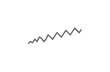
\begin{tikzpicture}[x=0.08em, y=0.08em, line width=0.4pt]
                \draw[FooterGray] (0,3) -- (1,4) -- (2,3.5) -- (3,5) -- (4,4) -- (5,6) -- (6,5.5) -- (7,4) -- (8,5) -- (9,7) -- (10,6) -- (11,5) -- (12,6.5) -- (13,8) -- (14,7) -- (15,6) -- (16,7.5) -- (17,9) -- (18,8) -- (19,7) -- (20,8.5) -- (21,10) -- (22,9) -- (23,8) -- (24,9.5);
            \end{tikzpicture}%
        }%
        \hskip0.5cm%
    }%
    \vskip6pt%
}

%=============================================================================
% PACHETE
%=============================================================================
\usepackage[utf8]{inputenc}
\usepackage[T1]{fontenc}
\usepackage{amsmath, amssymb, amsthm}
\usepackage{mathtools}
\usepackage{bm}
\usepackage{tikz}
\usetikzlibrary{arrows.meta, positioning, shapes, calc, decorations.pathreplacing, shadings}
\usepackage{booktabs}
\usepackage{multirow}
\usepackage{array}
\usepackage{graphicx}
\usepackage{hyperref}
\usepackage{colortbl}
\hypersetup{colorlinks=true, linkcolor=MainBlue, urlcolor=MainBlue}
\graphicspath{{../../logos/}{../../charts/}}
\hfuzz=2pt  % Suppress tiny overfull warnings (<2pt)
\vfuzz=2pt  % Suppress tiny vertical overfull warnings (<2pt)

%=============================================================================
% COMANDA QUANTLET
%=============================================================================
\newcommand{\quantlet}[2]{%
    \hfill\href{#2}{%
        \raisebox{-0.15em}{\includegraphics[height=0.7em]{ql_logo.png}}%
        \textcolor{MainBlue}{\tiny\ #1}%
    }%
}

%=============================================================================
% MEDII PENTRU TEOREME
%=============================================================================
\theoremstyle{definition}
\setbeamertemplate{theorems}[numbered]
\newtheorem{defn}{Definiție}
\newtheorem{thm}{Teoremă}
\newtheorem{prop}{Propoziție}
\newtheorem{rmk}{Observație}

%=============================================================================
% CENTRED MINIPAGE (fără spațiu vertical suplimentar)
%=============================================================================
\newenvironment{cminipage}[1]{%
    \par\noindent\hfill\begin{minipage}{#1}\ignorespaces
}{%
    \end{minipage}\hfill\null\par
}

%=============================================================================
% COMENZI PERSONALIZATE
%=============================================================================
\newcommand{\E}{\mathbb{E}}
\newcommand{\Var}{\text{Var}}
\newcommand{\Cov}{\text{Cov}}
\newcommand{\Corr}{\text{Corr}}
\newcommand{\R}{\mathbb{R}}
\newcommand{\N}{\mathbb{N}}
\newcommand{\Z}{\mathbb{Z}}
\newcommand{\B}{\mathbf{B}}
\newcommand{\imark}{\textcolor{MainBlue}{\textbullet}}
\newcommand{\RMSE}{\text{RMSE}}
\newcommand{\MAE}{\text{MAE}}
\newcommand{\MAPE}{\text{MAPE}}

%=============================================================================
% PAGINĂ TITLU PERSONALIZATĂ
%=============================================================================
\defbeamertemplate*{title page}{hybrid}[1][]
{
    \vspace{0.2cm}
    % Rând logo-uri - antet superior (cu linkuri clickabile)
    \begin{center}
        \href{https://www.ase.ro}{\includegraphics[height=1.0cm]{ase_logo.png}}\hspace{0.3cm}%
        \href{https://theida.net}{\includegraphics[height=1.0cm]{ida_logo.png}}\hspace{0.3cm}%
        \href{https://blockchain-research-center.com}{\includegraphics[height=1.0cm]{brc_logo.png}}\hspace{0.3cm}%
        \href{https://www.ai4efin.ase.ro}{\includegraphics[height=1.0cm]{ai4efin_logo.png}}\hspace{0.3cm}%
        \href{https://ipe.ro/new}{\includegraphics[height=1.0cm]{acad_logo.png}}\hspace{0.3cm}%
        \href{https://www.digital-finance-msca.com}{\includegraphics[height=1.0cm]{msca_logo.png}}%
    \end{center}

    \vspace{0.6cm}

    % Titlu principal cu logo-uri Q pe părți (cu linkuri clickabile)
    \begin{center}
        \begin{minipage}{0.1\textwidth}
            \centering
            \href{https://quantlet.com}{\includegraphics[height=1.1cm]{ql_logo.png}}
        \end{minipage}%
        \begin{minipage}{0.78\textwidth}
            \centering
            {\LARGE\bfseries\usebeamercolor[fg]{title}\inserttitle}

            \vspace{0.3cm}

            {\usebeamerfont{subtitle}\usebeamercolor[fg]{title}\insertsubtitle}
        \end{minipage}%
        \begin{minipage}{0.1\textwidth}
            \centering
            \href{https://quantinar.com}{\includegraphics[height=1.1cm]{qr_logo.png}}
        \end{minipage}
    \end{center}

    \vspace{0.6cm}

    % Autori (aliniere la stânga)
    \hspace{0.5cm}{\usebeamerfont{author}\insertauthor}

    \vspace{0.3cm}

    % Institut/Afilieri (aliniere la stânga)
    \hspace{0.5cm}\begin{minipage}[t]{0.95\textwidth}
        \raggedright\small\insertinstitute
    \end{minipage}
}

%=============================================================================
% INFORMAȚII TITLU
%=============================================================================
\title[Analiza Seriilor de Timp]{Analiza și Prognoza Seriilor de Timp}
\subtitle{Capitolul 4: Modele SARIMA pentru Serii de Timp Sezoniere}
\author[D.T. Pele]{Daniel Traian PELE}
\institute{Academia de Studii Economice din București\\
IDA Institute Digital Assets\\
Blockchain Research Center\\
AI4EFin Artificial Intelligence for Energy Finance\\
Academia Română, Institutul de Prognoză Economică\\
MSCA Digital Finance}
\date{}

\begin{document}

% Pagina de titlu (fără antet/subsol)
{
\setbeamertemplate{headline}{}
\setbeamertemplate{footline}{}
\begin{frame}
    \titlepage
\end{frame}
}

%=============================================================================
% OBIECTIVE DE ÎNVĂȚARE
%=============================================================================
\begin{frame}{Obiective de Învățare}
    {\small
    \begin{cminipage}{0.95\textwidth}
    \begin{block}{La finalul acestui capitol, veți fi capabili să:}
    \begin{enumerate}\setlength{\itemsep}{0pt}
        \item[\textcolor{MainBlue}{\textbf{1.}}] \textbf{Identificați} tiparele sezoniere în datele de tip serie de timp
        \item[\textcolor{MainBlue}{\textbf{2.}}] \textbf{Aplicați} diferențierea sezonieră pentru a elimina rădăcinile unitare sezoniere
        \item[\textcolor{MainBlue}{\textbf{3.}}] \textbf{Construiți} și estimați modele SARIMA cu componente sezoniere
        \item[\textcolor{MainBlue}{\textbf{4.}}] \textbf{Interpretați} tiparele ACF/PACF sezoniere pentru identificarea modelului
        \item[\textcolor{MainBlue}{\textbf{5.}}] \textbf{Evaluați} prognozele prin metoda ferestrei rolling pentru date sezoniere
        \item[\textcolor{MainBlue}{\textbf{6.}}] \textbf{Aplicați} metodologia completă pe date reale (pasageri aerieni)
    \end{enumerate}
    \end{block}
    \end{cminipage}
    }
\end{frame}

%=============================================================================
% SURSE DE DATE ȘI INSTRUMENTE SOFTWARE
%=============================================================================
\begin{frame}{Surse de date și instrumente software}
    \begin{cminipage}{0.95\textwidth}
    \begin{columns}[T]
        \begin{column}{0.48\textwidth}
            \begin{block}{Surse de date}
                \begin{itemize}\setlength{\itemsep}{0pt}
                    \item \textbf{FRED} (Federal Reserve)
                    \begin{itemize}
                        \item Vânzări cu amănuntul, producție industrială
                    \end{itemize}
                    \item \textbf{Yahoo Finance}
                    \begin{itemize}
                        \item Prețuri acțiuni, cursuri de schimb
                    \end{itemize}
                    \item \textbf{Eurostat / INS}
                    \begin{itemize}
                        \item Date macroeconomice sezoniere
                    \end{itemize}
                    \item \textbf{Statsmodels datasets}
                    \begin{itemize}
                        \item Airline passengers (Box-Jenkins)
                    \end{itemize}
                \end{itemize}
            \end{block}
        \end{column}
        \begin{column}{0.48\textwidth}
            \begin{exampleblock}{Python}
                \begin{itemize}\setlength{\itemsep}{0pt}
                    \item \texttt{statsmodels} --- modele SARIMA
                    \item \texttt{pmdarima} --- selecție automată
                    \item \texttt{pandas-datareader} --- descărcare FRED
                    \item \texttt{matplotlib} --- vizualizare
                    \item \texttt{scipy} --- teste statistice
                \end{itemize}
            \end{exampleblock}
            \begin{alertblock}{Resurse}
                \begin{itemize}\setlength{\itemsep}{0pt}
                    \item \href{https://github.com/QuantLet/TSA/tree/main/TSA_ch4}{\texttt{github.com/QuantLet/TSA/TSA\_ch4}}
                    \item \href{https://quantlet.com}{\texttt{quantlet.com}}
                \end{itemize}
            \end{alertblock}
        \end{column}
    \end{columns}
    \end{cminipage}
\end{frame}

%=============================================================================
% STRUCTURA CAPITOLULUI
%=============================================================================
\begin{frame}{Structura capitolului}
    \setbeamertemplate{section in toc}{\color{MainBlue}$\boxdot$~\inserttocsection}
    \tableofcontents
\end{frame}

%=============================================================================
% MOTIVAȚIE
%=============================================================================
\section{Motivație}

\begin{frame}{De ce SARIMA? Sezonalitatea este peste tot}
    \begin{cminipage}{0.95\textwidth}
    \vspace{-0.3cm}
    \begin{center}
        \includegraphics[width=0.88\textwidth, height=0.56\textheight, keepaspectratio]{ch4_motivation_seasonal.pdf}
    \end{center}
    \vspace{-0.2cm}
    {\footnotesize
    \begin{exampleblock}{}
    \begin{itemize}
        \item Vânzările cu amănuntul prezintă \textbf{tipare anuale} clare: vârfuri în decembrie, minime în ianuarie
        \item Modelele ARIMA standard nu pot captura aceste \textbf{cicluri sezoniere repetitive}
        \item Ignorarea sezonalității duce la erori sistematice de prognoză
    \end{itemize}
    \end{exampleblock}
    }
    \end{cminipage}
    \quantlet{TSA\_ch4\_motivation\_seasonal}{https://github.com/QuantLet/TSA/tree/main/TSA_ch4/TSA_ch4_motivation_seasonal}
\end{frame}

\begin{frame}{Înțelegerea componentelor sezoniere}
    \begin{cminipage}{0.95\textwidth}
    \vspace{-0.3cm}
    \begin{center}
        \includegraphics[width=0.88\textwidth, height=0.56\textheight, keepaspectratio]{ch4_motivation_decomposition.pdf}
    \end{center}
    \vspace{-0.2cm}
    {\footnotesize
    \begin{exampleblock}{}
    \begin{itemize}
        \item Serie de timp sezonieră = \textbf{Trend} + \textbf{Tipar sezonier} + \textbf{Reziduuri}
        \item Descompunerea ajută la vizualizarea separată a fiecărei componente
        \item Modelele SARIMA captează atât dinamica trendului, cât și comportamentul sezonier
    \end{itemize}
    \end{exampleblock}
    }
    \end{cminipage}
    \quantlet{TSA\_ch4\_motivation\_decomposition}{https://github.com/QuantLet/TSA/tree/main/TSA_ch4/TSA_ch4_motivation_decomposition}
\end{frame}

\begin{frame}{Aplicație reală: Tipare lunare}
    \begin{cminipage}{0.95\textwidth}
    \vspace{-0.3cm}
    \begin{center}
        \includegraphics[width=0.88\textwidth, height=0.56\textheight, keepaspectratio]{ch4_motivation_monthly.pdf}
    \end{center}
    \vspace{-0.2cm}
    {\footnotesize
    \begin{exampleblock}{}
    \begin{itemize}
        \item Cererea de energie prezintă o \textbf{sezonalitate lunară} puternică (cicluri de încălzire/răcire)
        \item Tiparul se repetă previzibil în fiecare an cu mici variații
        \item Companiile de utilități folosesc prognozele SARIMA pentru planificarea capacității
    \end{itemize}
    \end{exampleblock}
    }
    \end{cminipage}
    \quantlet{TSA\_ch4\_motivation\_monthly}{https://github.com/QuantLet/TSA/tree/main/TSA_ch4/TSA_ch4_motivation_monthly}
\end{frame}

\begin{frame}{De ce avem nevoie de SARIMA?}
    \begin{cminipage}{0.95\textwidth}
    \vspace{-0.3cm}
    \begin{center}
        \includegraphics[width=0.88\textwidth, height=0.57\textheight, keepaspectratio]{ch4_motivation_why_sarima.pdf}
    \end{center}
    \vspace{-0.2cm}
    {\footnotesize
    \begin{exampleblock}{}
    \begin{itemize}
        \item \textbf{Stânga}: ACF sezonieră prezintă vârfuri la lag-urile 12, 24, 36... (tipar anual)
        \item \textbf{Dreapta}: Reziduurile ARIMA încă prezintă autocorelație sezonieră $\succ$ modelul este incomplet
        \item SARIMA adaugă \textbf{termeni AR și MA sezonieri} pentru a captura aceste tipare
    \end{itemize}
    \end{exampleblock}
    }
    \end{cminipage}
    \quantlet{TSA\_ch4\_motivation\_why\_sarima}{https://github.com/QuantLet/TSA/tree/main/TSA_ch4/TSA_ch4_motivation_why_sarima}
\end{frame}

\begin{frame}{Ce vom învăța astăzi}
    \vspace{-0.2cm}
    {\small
    \begin{cminipage}{0.95\textwidth}
        \begin{columns}[T]
            \begin{column}{0.48\textwidth}
                \begin{block}{Concepte}
                    \begin{itemize}\setlength{\itemsep}{0pt}
                        \item Identificarea tiparelor sezoniere
                        \item Operatorul de diferențiere sezonieră
                        \item Notația SARIMA$(p,d,q)(P,D,Q)_s$
                        \item Celebrul ``Model Airline''
                        \item Selecția modelului pentru date sezoniere
                    \end{itemize}
                \end{block}
            \end{column}
            \begin{column}{0.48\textwidth}
                \begin{block}{Abilități}
                    \begin{itemize}\setlength{\itemsep}{0pt}
                        \item Detectarea sezonalității din ACF/PACF
                        \item Determinarea perioadei sezoniere $s$
                        \item Alegerea ordinelor sezoniere $(P, D, Q)$
                        \item Implementarea SARIMA în Python/R
                        \item Prognoza seriilor de timp sezoniere
                    \end{itemize}
                \end{block}
            \end{column}
        \end{columns}

    \vspace{0.05cm}

    \begin{alertblock}{Ideea cheie}
        \begin{itemize}\setlength{\itemsep}{0pt}
            \item SARIMA = ARIMA aplicată la \textbf{două frecvențe}: non-sezonieră (termen scurt) și sezonieră (termen lung)
        \end{itemize}
    \end{alertblock}
    \end{cminipage}
    }
\end{frame}

%=============================================================================
% SECȚIUNEA 1: SEZONALITATEA ÎN SERIILE DE TIMP
%=============================================================================
\section{Sezonalitatea în seriile de timp}

\begin{frame}{Ce este sezonalitatea?}
    \vspace{-0.2cm}
    \begin{columns}[T]
        \column{0.55\textwidth}
        {\scriptsize
        \begin{cminipage}{0.95\textwidth}
        \begin{defn}[Sezonalitate]
            \begin{itemize}\setlength{\itemsep}{0pt}
                \item O serie de timp prezintă \textbf{sezonalitate} când arată fluctuații regulate, periodice care se repetă pe o perioadă fixă $s$ (perioadă sezonieră)
            \end{itemize}
        \end{defn}

        \vspace{0.1cm}

        \begin{exampleblock}{Perioade sezoniere comune}
            \begin{itemize}
                \item Date lunare: $s = 12$ (ciclu anual)
                \item Date trimestriale: $s = 4$ (ciclu anual)
                \item Date săptămânale: $s = 52$ (anual) sau $s = 7$ (tipar săptămânal)
                \item Date zilnice: $s = 7$ (tipar săptămânal)
            \end{itemize}
        \end{exampleblock}
        \end{cminipage}
        }
        \column{0.43\textwidth}
        \vspace{-0.3cm}
        \begin{center}
            \includegraphics[width=\textwidth, keepaspectratio]{ch4_def_seasonality.pdf}
        \end{center}
        \quantlet{TSA\_ch4\_seasonality}{https://github.com/QuantLet/TSA/tree/main/TSA_ch4/TSA_ch4_seasonality}
    \end{columns}
\end{frame}

\begin{frame}{Exemple de date sezoniere}
    {\small
    \begin{cminipage}{0.95\textwidth}
    \begin{columns}[T]
        \begin{column}{0.48\textwidth}
            \begin{block}{Serii economice}
                \begin{itemize}\setlength{\itemsep}{0pt}
                    \item Vânzări cu amănuntul (vârfuri de sărbători)
                    \item Turism (vara/iarna)
                    \item Producție agricolă
                    \item Consum de energie
                    \item Ocuparea forței de muncă (cicluri de angajare)
                \end{itemize}
            \end{block}
        \end{column}
        \begin{column}{0.48\textwidth}
            \begin{block}{Alte domenii}
                \begin{itemize}\setlength{\itemsep}{0pt}
                    \item Vreme/temperatură
                    \item Trafic pe site-uri web
                    \item Admisii la spital
                    \item Utilizarea transportului
                    \item Cererea de electricitate
                \end{itemize}
            \end{block}
        \end{column}
    \end{columns}

    \begin{alertblock}{De ce contează}
        \begin{itemize}\setlength{\itemsep}{0pt}
            \item Ignorarea sezonalității duce la prognoze distorsionate și inferență invalidă!
        \end{itemize}
    \end{alertblock}
    \end{cminipage}
    }
\end{frame}

\begin{frame}{Exemplu: Datele privind pasagerii companiilor aeriene}
    \begin{cminipage}{0.95\textwidth}
    \vspace{-0.3cm}
    \begin{center}
        \includegraphics[width=0.88\textwidth, height=0.56\textheight, keepaspectratio]{ch4_airline_data.pdf}
    \end{center}
    \vspace{-0.2cm}
    {\footnotesize
    \begin{exampleblock}{}
    \begin{itemize}
        \item Pasageri internaționali lunari (1949--1960)
        \item \textbf{Trend ascendent} clar și \textbf{amplitudine sezonieră crescătoare}
        \item Vârfurile din vară reflectă tiparele călătoriilor de vacanță
    \end{itemize}
    \end{exampleblock}
    }
    \end{cminipage}
    \quantlet{TSA\_ch4\_airline\_data}{https://github.com/QuantLet/TSA/tree/main/TSA_ch4/TSA_ch4_airline_data}
\end{frame}

\begin{frame}{Vizualizarea tiparelor sezoniere}
    \begin{cminipage}{0.95\textwidth}
    \vspace{-0.3cm}
    \begin{center}
        \includegraphics[width=0.88\textwidth, height=0.56\textheight, keepaspectratio]{ch4_seasonal_boxplot.pdf}
    \end{center}
    \vspace{-0.2cm}
    {\footnotesize
    \begin{exampleblock}{}
    \begin{itemize}
        \item Diagrama box plot relevă un tipar sezonier consistent
        \item Iulie--August: cele mai mari numere de pasageri (călătorii de vară)
        \item Noiembrie--Februarie: cele mai mici numere (lunile de iarnă)
    \end{itemize}
    \end{exampleblock}
    }
    \end{cminipage}
    \quantlet{TSA\_ch4\_seasonal\_boxplot}{https://github.com/QuantLet/TSA/tree/main/TSA_ch4/TSA_ch4_seasonal_boxplot}
\end{frame}

\begin{frame}{Sezonalitate deterministă vs stochastică}
    \vspace{-0.2cm}
    {\footnotesize
    \begin{cminipage}{0.95\textwidth}
    \begin{columns}[T]
        \begin{column}{0.48\textwidth}
            \begin{block}{Sezonalitate deterministă}
                \begin{itemize}\setlength{\itemsep}{0pt}
                    \item \textbf{Tipar fix}: $Y_t = \sum_{j=1}^{s} \gamma_j D_{jt} + \varepsilon_t$
                    \begin{itemize}
                        \item $D_{jt}$ sunt variabile dummy sezoniere
                    \end{itemize}
                    \item Tiparul constant în timp
                    \item Aceeași amplitudine în fiecare an
                    \item Eliminare prin regresie pe dummy-uri
                    \item ACF: scădere bruscă la lag-uri sezoniere
                    \item \textbf{Exemplu:} Înscrierile universitare cresc în fiecare septembrie cu aceeași valoare
                \end{itemize}
            \end{block}
        \end{column}
        \begin{column}{0.48\textwidth}
            \begin{block}{Sezonalitate stochastică}
                \begin{itemize}\setlength{\itemsep}{0pt}
                    \item \textbf{Tipar în evoluție}: $\Delta_s Y_t = Y_t - Y_{t-s}$
                    \begin{itemize}
                        \item Prezintă structură de dependență
                    \end{itemize}
                    \item Tiparul evoluează în timp
                    \item Amplitudinea poate crește sau scădea
                    \item Necesită diferențiere sezonieră
                    \item ACF: scădere lentă la lag-uri sezoniere
                    \item \textbf{Exemplu:} Vânzările de retail cresc tot mai mult în fiecare decembrie
                \end{itemize}
            \end{block}
        \end{column}
    \end{columns}

    \vspace{0.05cm}

    \begin{alertblock}{Cum decidem?}
        \begin{itemize}\setlength{\itemsep}{0pt}
            \item Scădere lentă a ACF la lag-urile $s, 2s, 3s, \ldots$ $\Rightarrow$ stochastică (folosiți $\Delta_s$)
            \item Scădere bruscă $\Rightarrow$ deterministă (folosiți dummy-uri)
            \item Confirmați cu testele HEGY sau Canova-Hansen
        \end{itemize}
    \end{alertblock}
    \end{cminipage}
    }
\end{frame}

\begin{frame}{Sezonalitate aditivă vs multiplicativă}
    \begin{cminipage}{0.95\textwidth}
    {\scriptsize
    \begin{columns}[T]
        \column{0.48\textwidth}
        \begin{block}{Aditivă: $Y_t = T_t + S_t + \varepsilon_t$}
            \vspace{-2pt}
            \begin{itemize}\setlength{\itemsep}{0pt}
                \item Amplitudinea sezonieră \textbf{constantă}
                \item Nu necesită transformare
                \item Ex: temperaturi, înscrieri universitare
            \end{itemize}
            \vspace{-2pt}
        \end{block}
        \column{0.48\textwidth}
        \begin{block}{Multiplicativă: $Y_t = T_t \cdot S_t \cdot \varepsilon_t$}
            \vspace{-2pt}
            \begin{itemize}\setlength{\itemsep}{0pt}
                \item Amplitudinea \textbf{crește cu nivelul}
                \item Necesită transformare log (Box-Cox)
                \item Ex: Airline, vânzări retail, PIB
            \end{itemize}
            \vspace{-2pt}
        \end{block}
    \end{columns}
    }
    \vspace{-0.1cm}
    {\footnotesize
    \begin{alertblock}{Prima decizie practică}
        \vspace{-2pt}
        \begin{itemize}\setlength{\itemsep}{0pt}
            \item Amplitudinea crește cu trendul? $\Rightarrow$ multiplicativă $\Rightarrow$ aplicați log/Box-Cox \textit{înainte} de diferențiere
        \end{itemize}
        \vspace{-2pt}
    \end{alertblock}
    }
    \end{cminipage}
\end{frame}

\begin{frame}{Sezonalitate aditivă vs multiplicativă}
    \begin{center}
        \includegraphics[width=0.95\textwidth, height=0.78\textheight, keepaspectratio]{additive_vs_multiplicative.pdf}
    \end{center}
\end{frame}

\begin{frame}{Detectarea sezonalității}
    \vspace{-0.2cm}
    {\small
    \begin{cminipage}{0.95\textwidth}
    \begin{block}{Metode vizuale}
        \begin{itemize}\setlength{\itemsep}{0pt}
            \item Graficul seriei de timp -- căutați tipare repetitive
            \item Graficul sub-seriilor sezoniere -- comparați aceleași sezoane de-a lungul anilor
            \item Graficul ACF -- vârfuri la lag-uri sezoniere ($s, 2s, 3s, \ldots$)
        \end{itemize}
    \end{block}
    \vspace{-0.1cm}
    \begin{block}{Teste statistice}
        \begin{itemize}\setlength{\itemsep}{0pt}
            \item Teste de rădăcină unitară sezonieră (HEGY, Canova-Hansen, OCSB\footnote{\scriptsize Osborn-Chui-Smith-Birchenhall --- testul implicit din \texttt{auto\_arima}})
            \item Testul F pentru variabile dummy sezoniere
            \item Testul Kruskal-Wallis (neparametric)
        \end{itemize}
    \end{block}
    \vspace{-0.1cm}
    \begin{exampleblock}{Semnatura ACF}
        \begin{itemize}\setlength{\itemsep}{0pt}
            \item Sezonalitate puternică: ACF prezintă vârfuri semnificative la lag-urile $s, 2s, 3s, \ldots$
        \end{itemize}
    \end{exampleblock}
    \end{cminipage}
    }
\end{frame}

\begin{frame}{ACF relevă structura sezonieră}
    \begin{cminipage}{0.95\textwidth}
    \vspace{-0.3cm}
    \begin{center}
        \includegraphics[width=0.88\textwidth, height=0.58\textheight, keepaspectratio]{ch4_acf_seasonality.pdf}
    \end{center}
    \vspace{-0.2cm}
    {\footnotesize
    \begin{exampleblock}{}
    \begin{itemize}
        \item \textbf{Descreștere lentă} la toate lag-urile indică nestaționaritate (trend)
        \item \textbf{Vârfuri la lag-urile 12, 24, 36} confirmă tiparul sezonier ($s=12$)
        \item ACF la lag-urile sezoniere: descreștere lentă $\succ$ necesită diferențiere sezonieră
    \end{itemize}
    \end{exampleblock}
    }
    \end{cminipage}
    \quantlet{TSA\_ch4\_acf\_seasonality}{https://github.com/QuantLet/TSA/tree/main/TSA_ch4/TSA_ch4_acf_seasonality}
\end{frame}

\begin{frame}{Testul F pentru variabile dummy sezoniere: intuiție}
    \vspace{-0.2cm}
    {\footnotesize
    \begin{cminipage}{0.95\textwidth}
    \begin{block}{Ce face acest test?}
        \begin{itemize}\setlength{\itemsep}{0pt}
            \item \textbf{Scop}: testează dacă valorile medii diferă semnificativ între sezoane
            \item \textbf{Logică}: dacă media din ianuarie $\neq$ media din februarie $\neq$ \ldots $\neq$ media din decembrie $\succ$ sezonalitate
            \item \textbf{Metodă}: compară un model CU variabile dummy sezoniere vs. un model FĂRĂ
        \end{itemize}
    \end{block}
    \vspace{-0.1cm}
    \begin{block}{Modelele comparate}
        \begin{itemize}\setlength{\itemsep}{0pt}
            \item \textbf{Restricționat}: $Y_t = \alpha + \varepsilon_t$ \quad \textbf{Nerestricționat}: $Y_t = \alpha + \sum_{j=1}^{s-1} \gamma_j D_{jt} + \varepsilon_t$
            \item unde $D_{jt} = 1$ dacă observația $t$ este în sezonul $j$, 0 altfel
        \end{itemize}
    \end{block}
    \vspace{-0.1cm}
    \begin{alertblock}{Ideea cheie}
        \begin{itemize}\setlength{\itemsep}{0pt}
            \item Dacă adăugarea dummy sezoniere \textbf{reduce semnificativ} erorile de predicție $\succ$ sezonalitate prezentă
        \end{itemize}
    \end{alertblock}
    \end{cminipage}
    }
\end{frame}

\begin{frame}{Testul F pentru variabile dummy sezoniere: formula și exemplu}
    {\small
    \begin{cminipage}{0.95\textwidth}
    \begin{block}{Formula statisticii F}
        \begin{itemize}\setlength{\itemsep}{0pt}
            \item \textbf{Formula}: $F = \frac{(SSR_R - SSR_U)/(s-1)}{SSR_U/(n-s)} \sim F_{s-1, n-s}$
            \begin{itemize}\setlength{\itemsep}{0pt}
                \item \textbf{$SSR_R$}: suma pătratelor reziduurilor din modelul restricționat (fără dummy)
                \item \textbf{$SSR_U$}: suma pătratelor reziduurilor din modelul nerestricționat (cu dummy)
                \item \textbf{$s-1$}: numărul de restricții (lunar: 11, trimestrial: 3)
            \end{itemize}
        \end{itemize}
    \end{block}

    \begin{exampleblock}{Exemplu numeric (Date lunare, n=120)}
        \begin{itemize}\setlength{\itemsep}{0pt}
            \item $SSR_R = 15000$, $SSR_U = 8500$, $s = 12$
            \item $F = \frac{(15000 - 8500)/11}{8500/108} = \frac{590.9}{78.7} = 7.51$
            \item Valoare critică $F_{0.05, 11, 108} \approx 1.87$. Cum $7.51 > 1.87$: \textbf{Respingem $H_0$} $\Rightarrow$ Sezonalitate!
        \end{itemize}
    \end{exampleblock}
    \end{cminipage}
    }
\end{frame}

\begin{frame}{Testul Kruskal-Wallis: intuiție}
    \vspace{-0.2cm}
    {\small
    \begin{cminipage}{0.95\textwidth}
    \begin{block}{Ce face acest test?}
        \begin{itemize}\setlength{\itemsep}{0pt}
            \item \textbf{Test neparametric}: verifică dacă observațiile din diferite sezoane provin din aceeași distribuție
            \item \textbf{Mecanism}: ordonează toate observațiile de la cea mai mică la cea mai mare
            \item \textbf{Verificare}: dacă rangurile sunt distribuite uniform între sezoane
            \item \textbf{Concluzie}: dacă un sezon are constant ranguri mai mari/mici $\succ$ sezonalitate
        \end{itemize}
    \end{block}

    \vspace{0.05cm}

    \begin{exampleblock}{De ce să-l folosim în locul testului F?}
        \begin{itemize}\setlength{\itemsep}{0pt}
            \item \textbf{Fără ipoteza de normalitate} -- funcționează cu orice distribuție
            \item \textbf{Robust la valori extreme} -- valorile extreme nu distorsionează rezultatele
        \end{itemize}
    \end{exampleblock}

    \vspace{0.05cm}

    \begin{alertblock}{Limitare}
        \begin{itemize}\setlength{\itemsep}{0pt}
            \item Mai puțin puternic decât testul F când datele SUNT distribuite normal
        \end{itemize}
    \end{alertblock}
    \end{cminipage}
    }
\end{frame}

\begin{frame}{Testul Kruskal-Wallis: formula și exemplu}
    \vspace{-0.2cm}
    {\footnotesize
    \begin{cminipage}{0.95\textwidth}
    \begin{block}{Statistică de test}
        \begin{itemize}\setlength{\itemsep}{0pt}
            \item $H = \frac{12}{N(N+1)} \sum_{j=1}^{s} \frac{R_j^2}{n_j} - 3(N+1)$ \quad unde $N$ = total obs., $n_j$ = obs. în sezonul $j$, $R_j$ = suma rangurilor
        \end{itemize}
    \end{block}
    \vspace{-0.1cm}
    \begin{exampleblock}{Exemplu: Vânzări trimestriale (n=20, s=4)}
        \begin{itemize}\setlength{\itemsep}{0pt}
            \item Date ordonate 1-20. Sumele rangurilor: T1: $R_1 = 15$, T2: $R_2 = 35$, T3: $R_3 = 70$, T4: $R_4 = 90$
            \item $H = \frac{12}{20 \times 21}\left(\frac{15^2}{5} + \frac{35^2}{5} + \frac{70^2}{5} + \frac{90^2}{5}\right) - 3(21) = 19.6$
            \item Valoarea critică $\chi^2_{0.05, 3} = 7.81$. Deoarece $19.6 > 7.81$: \textbf{Respingem $H_0$} $\succ$ Sezonalitate!
        \end{itemize}
    \end{exampleblock}
    \vspace{-0.1cm}
    \begin{alertblock}{În Python}
        \begin{itemize}\setlength{\itemsep}{0pt}
            \item \textbf{Implementare}: \texttt{scipy.stats.kruskal(q1, q2, q3, q4)}
        \end{itemize}
    \end{alertblock}
    \end{cminipage}
    }
\end{frame}

\begin{frame}{Testul HEGY: ce problemă rezolvă?}
    \vspace{-0.3cm}
    {\footnotesize
    \begin{cminipage}{0.95\textwidth}
    \begin{block}{Întrebarea cheie}
        \begin{itemize}\setlength{\itemsep}{0pt}
            \item \textbf{Problemă}: având o serie sezonieră, trebuie să știm tipul de diferențiere
            \item \textbf{Diferențiere obișnuită} $(1-L)$? $\succ$ setăm $d=1$; \textbf{Diferențiere sezonieră} $(1-L^s)$? $\succ$ setăm $D=1$
            \item \textbf{HEGY}: testează pentru ambele tipuri de rădăcini unitare simultan!
        \end{itemize}
    \end{block}
    \vspace{-0.1cm}
    \begin{exampleblock}{De ce să nu folosim doar ADF?}
        \begin{itemize}\setlength{\itemsep}{0pt}
            \item \textbf{ADF}: testează doar pentru o rădăcină unitară obișnuită la frecvența zero
            \item \textbf{Limitare}: datele sezoniere pot avea rădăcini unitare la frecvențe sezoniere pe care ADF le omite!
        \end{itemize}
    \end{exampleblock}
    \vspace{-0.1cm}
    \begin{alertblock}{HEGY testează frecvențe multiple}
        \begin{itemize}\setlength{\itemsep}{0pt}
            \item \textbf{Trimestrial}: testează la 0, $\pi$, $\pm\pi/2$
            \item \textbf{Lunar}: testează la 0, $\pi$, $\pm\pi/6$, $\pm\pi/3$, $\pm\pi/2$, $\pm 2\pi/3$, $\pm 5\pi/6$
        \end{itemize}
    \end{alertblock}
    \end{cminipage}
    }
\end{frame}

\begin{frame}{Testul HEGY: Formula de regresie (Trimestrial)}
    \vspace{-0.3cm}
    {\footnotesize
    \begin{cminipage}{0.95\textwidth}
    \begin{block}{Regresia auxiliară HEGY}
        \begin{itemize}\setlength{\itemsep}{0pt}
            \item \textbf{Date trimestriale} ($s=4$): $\Delta_4 y_t = \pi_1 z_{1,t-1} + \pi_2 z_{2,t-1} + \pi_3 z_{3,t-2} + \pi_4 z_{4,t-2} + \sum_{j=1}^{k} \phi_j \Delta_4 y_{t-j} + \varepsilon_t$
        \end{itemize}
    \end{block}
    \vspace{-0.15cm}
    \begin{block}{Variabile transformate}
        \begin{itemize}\setlength{\itemsep}{0pt}
            \item \textbf{$z_{1t}$}: $(1+L+L^2+L^3)y_t = y_t + y_{t-1} + y_{t-2} + y_{t-3}$
            \item \textbf{$z_{2t}$}: $-(1-L+L^2-L^3)y_t = -y_t + y_{t-1} - y_{t-2} + y_{t-3}$
            \item \textbf{$z_{3t}$}: $-(1-L^2)y_t = -y_t + y_{t-2}$
            \item \textbf{$z_{4t}$}: $-(L-L^3)y_t = -y_{t-1} + y_{t-3}$
        \end{itemize}
    \end{block}
    \vspace{-0.15cm}
    \begin{alertblock}{Ipoteze}
        \begin{itemize}\setlength{\itemsep}{0pt}
            \item \textbf{$H_0: \pi_1=0$}: rădăcină unitară la frecvența 0; \textbf{$H_0: \pi_2=0$}: la frecvența $\pi$
            \item \textbf{$H_0: \pi_3=\pi_4=0$}: rădăcină unitară la frecvența $\pm\pi/2$
        \end{itemize}
    \end{alertblock}
    \end{cminipage}
    }
\end{frame}

\begin{frame}{Testul HEGY: Reguli de decizie cu exemple}
    \vspace{-0.3cm}
    {\footnotesize
    \begin{cminipage}{0.95\textwidth}
    \begin{block}{Valori critice HEGY (5\%, n=100, cu constanta)}
        \begin{center}
        \resizebox{\linewidth}{!}{%
        \begin{tabular}{lccc}
            \toprule
            Test & Statistică & Valoare critică & Dacă NU este respins... \\
            \midrule
            $t_1$ ($\pi_1=0$) & t-stat & $-2.88$ & Necesită $d=1$ \\
            $t_2$ ($\pi_2=0$) & t-stat & $-2.88$ & Necesită $D=1$ \\
            $F_{34}$ ($\pi_3=\pi_4=0$) & F-stat & $6.57$ & Necesită $D=1$ \\
            \bottomrule
        \end{tabular}}
        \end{center}
    \end{block}

    \begin{exampleblock}{Exemplu: PIB trimestrial}
        \begin{itemize}\setlength{\itemsep}{0pt}
            \item \textbf{Rezultate HEGY}: $t_1 = -1.52$, $t_2 = -4.21$, $F_{34} = 2.15$
            \item $t_1 = -1.52 > -2.88$: Nu putem respinge $\succ$ \textbf{necesită $d=1$}
            \item $t_2 = -4.21 < -2.88$: Respingem $\succ$ fără rădăcină unitară la $\pi$
            \item $F_{34} = 2.15 < 6.57$: Nu putem respinge $\succ$ \textbf{necesită $D=1$}
            \item \textbf{Concluzie}: Folosim SARIMA cu $d=1, D=1$
        \end{itemize}
    \end{exampleblock}
    \end{cminipage}
    }
\end{frame}

\begin{frame}{Testul Canova-Hansen: opusul testului HEGY}
    \vspace{-0.2cm}
    {\footnotesize
    \begin{cminipage}{0.95\textwidth}
    \begin{block}{HEGY vs Canova-Hansen: Ipoteze nule diferite!}
        \begin{center}
        \resizebox{\linewidth}{!}{%
        \begin{tabular}{lcc}
            \toprule
            & \textbf{HEGY} & \textbf{Canova-Hansen} \\
            \midrule
            $H_0$ & Rădăcină unitară sezonieră & \textbf{Fără} rădăcină unitară sezonieră \\
            $H_1$ & Fără rădăcină unitară sezonieră & Rădăcină unitară sezonieră \\
            \midrule
            Respingem $H_0$ & Folosim variabile dummy sezoniere & Folosim diferențiere $(1-L^s)$ \\
            Nu respingem & Folosim diferențiere $(1-L^s)$ & Folosim variabile dummy sezoniere \\
            \bottomrule
        \end{tabular}}
        \end{center}
    \end{block}

    \begin{alertblock}{De ce contează?}
        \begin{itemize}\setlength{\itemsep}{0pt}
            \item HEGY: ``Demonstrați că NU există rădăcină unitară'' (conservator față de diferențiere)
            \item CH: ``Demonstrați că EXISTĂ rădăcină unitară'' (conservator față de variabile dummy)
            \item Folosiți \textbf{ambele} teste pentru concluzii robuste!
        \end{itemize}
    \end{alertblock}
    \end{cminipage}
    }
\end{frame}

\begin{frame}{Testul Canova-Hansen: formula}
    \vspace{-0.2cm}
    {\footnotesize
    \begin{cminipage}{0.95\textwidth}
    \begin{block}{Procedura de testare}
        \begin{itemize}\setlength{\itemsep}{0pt}
            \item \textbf{Pas 1}: Regresam $y_t$ pe variabile dummy sezoniere: $y_t = \sum_{j=1}^{s} \gamma_j D_{jt} + u_t$
            \item \textbf{Pas 2}: Calculam sumele parțiale la frecvența sezonieră $\lambda_i$:
            \begin{itemize}
                \item $S_{it}^{(c)} = \sum_{j=1}^{t} \hat{u}_j \cos(\lambda_i j)$, \; $S_{it}^{(s)} = \sum_{j=1}^{t} \hat{u}_j \sin(\lambda_i j)$
            \end{itemize}
        \end{itemize}
    \end{block}
    \vspace{-0.15cm}
    \begin{block}{Statistică de test LM}
        \begin{itemize}\setlength{\itemsep}{0pt}
            \item $LM_i = \frac{1}{T^2 \hat{\omega}_i} \left[ \sum_{t=1}^{T} (S_{it}^{(c)})^2 + \sum_{t=1}^{T} (S_{it}^{(s)})^2 \right]$
            \item unde $\hat{\omega}_i$ = estimator consistent al densității spectrale la frecvența $\lambda_i$
        \end{itemize}
    \end{block}
    \vspace{-0.15cm}
    \begin{alertblock}{Decizie}
        \begin{itemize}\setlength{\itemsep}{0pt}
            \item \textbf{Regula}: respingem $H_0$ dacă $LM > $ valoare critică $\succ$ necesară diferențierea sezonieră
        \end{itemize}
    \end{alertblock}
    \end{cminipage}
    }
\end{frame}

\begin{frame}{Sumar: Alegerea testului de sezonalitate potrivit}
    \vspace{-0.2cm}
    {\footnotesize
    \begin{cminipage}{0.95\textwidth}
    \begin{block}{Comparație teste de sezonalitate}
        \begin{center}
        \resizebox{\linewidth}{!}{%
        \begin{tabular}{p{2cm}p{2.5cm}p{2.5cm}p{3cm}}
            \toprule
            \textbf{Test} & \textbf{$H_0$} & \textbf{Dacă respingem} & \textbf{Cel mai bun pentru} \\
            \midrule
            Test F & Fără sezonalitate & Sezonalitate există & Date normale \\
            Kruskal-Wallis & Fără diferență între sezoane & Sezonalitate există & Non-normale, valori extreme \\
            HEGY & Rădăcină unitară există & Folosim dummy & Determinarea $d$, $D$ \\
            Canova-Hansen & Fără rădăcină unitară & Folosim $(1-L^s)$ & Confirmarea stabilității \\
            \bottomrule
        \end{tabular}}
        \end{center}
    \end{block}

    \begin{alertblock}{Ideea cheie}
        \vspace{-2pt}
        \begin{itemize}\setlength{\itemsep}{0pt}
            \item \textbf{Test F/Kruskal-Wallis}: ``\textit{Există sezonalitate?}'' \quad \textbf{HEGY/CH}: ``\textit{Ce tip?}'' (deterministă vs stochastică)
            \item \textbf{În practică}: pentru serii cu sezonalitate evidentă, boxplot + ACF sunt suficiente; testele formale sunt esențiale când sezonalitatea e ambiguă
        \end{itemize}
        \vspace{-2pt}
    \end{alertblock}
    \end{cminipage}
    }
\end{frame}

%=============================================================================
% TRANSFORMAREA BOX-COX
%=============================================================================

\begin{frame}{Transformarea Box-Cox: Stabilizarea varianței}
    \vspace{-0.2cm}
    {\footnotesize
    \begin{cminipage}{0.95\textwidth}
    \begin{block}{Familia de transformări Box-Cox}
        \begin{itemize}\setlength{\itemsep}{0pt}
            \item \textbf{Formula}: $Y_t^{(\lambda)} = \begin{cases} \frac{Y_t^\lambda - 1}{\lambda} & \text{dacă } \lambda \neq 0 \\ \ln(Y_t) & \text{dacă } \lambda = 0 \end{cases}$
            \item \textbf{Cazuri speciale}: $\lambda=1$ (fără transformare), $\lambda=0$ (logaritm), $\lambda=0.5$ (rădăcină pătrată)
        \end{itemize}
    \end{block}
    \vspace{-0.1cm}
    \begin{exampleblock}{Selectarea automată a lui $\lambda$}
        \begin{itemize}\setlength{\itemsep}{0pt}
            \item \textbf{Verosimilitate profilată}: maximizează log-verosimilitatea în funcție de $\lambda$
            \item \textbf{Metoda Guerrero (1993)}: minimizează coeficientul de variație al sub-seriilor sezoniere
            \item \textbf{Python}: \texttt{boxcox(y)} din \texttt{scipy.stats} sau \texttt{BoxCox.lambda\_(y)} din R
        \end{itemize}
    \end{exampleblock}
    \vspace{-0.1cm}
    \begin{alertblock}{De ce nu doar logaritm?}
        \begin{itemize}\setlength{\itemsep}{0pt}
            \item Log ($\lambda=0$) presupune varianță proporțională cu nivelul --- nu este întotdeauna cazul
            \item Box-Cox alege transformarea optimală bazat pe date, nu pe ipoteze
        \end{itemize}
    \end{alertblock}
    \end{cminipage}
    }
\end{frame}

\begin{frame}{Box-Cox pe datele Airline: Exemplu complet}
    \begin{cminipage}{0.95\textwidth}
    {\footnotesize
    \begin{columns}[T]
        \column{0.48\textwidth}
        \begin{exampleblock}{Rezultat pentru Airline Passengers}
            \begin{itemize}\setlength{\itemsep}{0pt}
                \item $\hat{\lambda} = 0.148 \approx 0$ $\Rightarrow$ log e aproape optim
                \item Abaterea standard pe an: de la crescătoare (original) la stabilă (log)
            \end{itemize}
        \end{exampleblock}
        \column{0.48\textwidth}
        \begin{alertblock}{Corecția de bias la back-transformare}
            \begin{itemize}\setlength{\itemsep}{0pt}
                \item Pe scara log: $\hat{y}_{T+h}$ este \textbf{mediana}, nu media
                \item Corecție: $\hat{Y}_{T+h} = \exp\!\left(\hat{y}_{T+h} + \frac{\sigma^2_h}{2}\right)$
                \item Fără corecție: prognoze sistematic sub-estimate!
            \end{itemize}
        \end{alertblock}
    \end{columns}
    }
    \end{cminipage}
\end{frame}

\begin{frame}{Box-Cox pe datele Airline: Exemplu complet}
    \begin{center}
        \includegraphics[width=0.95\textwidth, height=0.78\textheight, keepaspectratio]{ch4_boxcox_airline.pdf}
    \end{center}
    \quantlet{TSA\_ch4\_boxcox\_airline}{https://github.com/QuantLet/TSA/tree/main/TSA_ch4/TSA_ch4_boxcox_airline}
\end{frame}

\begin{frame}{Descompunerea STL: Alternative moderne}
    {\scriptsize
    \begin{cminipage}{0.95\textwidth}
    \begin{block}{STL: Seasonal-Trend decomposition using Loess (Cleveland et al., 1990)}
        \vspace{-2pt}
        \begin{itemize}\setlength{\itemsep}{0pt}
            \item \textbf{Avantaje}: sezonalitate variabilă în timp, robustă la outliers, orice perioadă $s$
            \item \textbf{Algoritm}: regresie locală ponderată (loess) iterativă
        \end{itemize}
        \vspace{-2pt}
    \end{block}

    \begin{exampleblock}{Parametri cheie}
        \vspace{-2pt}
        \begin{itemize}\setlength{\itemsep}{0pt}
            \item \textbf{Fereastra sezonieră} (\texttt{seasonal}): controlează cât de rapid se schimbă sezonalitatea
            \item \textbf{Fereastra de trend} (\texttt{trend}): netezirea componentei de trend
            \item \textbf{Robustitate} (\texttt{robust=True}): reduce influența outlier-ilor
        \end{itemize}
        \vspace{-2pt}
    \end{exampleblock}

    \begin{alertblock}{Utilizare practică}
        \vspace{-2pt}
        \begin{itemize}\setlength{\itemsep}{0pt}
            \item STL pentru explorare și pre-procesare; SARIMA pentru modelare și prognoză
            \item Python: \texttt{STL(y, period=12).fit()} din \texttt{statsmodels}
        \end{itemize}
        \vspace{-2pt}
    \end{alertblock}
    \end{cminipage}
    }
\end{frame}

%=============================================================================
% SECȚIUNEA 2: DIFERENȚIEREA SEZONIERĂ
%=============================================================================
\section{Diferențierea sezonieră}

\begin{frame}{Operatorul de diferență sezonieră}
    \begin{cminipage}{0.95\textwidth}
    \begin{defn}[Diferență sezonieră]
        \begin{itemize}\setlength{\itemsep}{0pt}
            \item \textbf{Operatorul de diferență sezonieră} $\Delta_s$ este definit ca:
            $$\Delta_s Y_t = (1 - L^s) Y_t = Y_t - Y_{t-s}$$
            \item unde $L^s Y_t = Y_{t-s}$ este operatorul de lag sezonier
        \end{itemize}
    \end{defn}

    \vspace{0.1cm}

    \begin{exampleblock}{Exemple}
        \begin{itemize}\setlength{\itemsep}{0pt}
            \item \textbf{Date lunare} ($s=12$): $\Delta_{12} Y_t = Y_t - Y_{t-12}$
            \begin{itemize}
                \item Compară fiecare lună cu aceeași lună din anul trecut
            \end{itemize}
            \item \textbf{Date trimestriale} ($s=4$): $\Delta_4 Y_t = Y_t - Y_{t-4}$
            \begin{itemize}
                \item Compară fiecare trimestru cu același trimestru din anul trecut
            \end{itemize}
        \end{itemize}
    \end{exampleblock}
    \end{cminipage}
\end{frame}

\begin{frame}{Diferența sezonieră: Ilustrare vizuală}
    \begin{cminipage}{0.95\textwidth}
    \vspace{-0.3cm}
    \begin{center}
        \includegraphics[width=0.88\textwidth, height=0.62\textheight, keepaspectratio]{ch4_def_seasonal_diff.pdf}
    \end{center}
    \vspace{-0.2cm}
    {\footnotesize
    \begin{exampleblock}{}
    \begin{itemize}
        \item \textbf{Stânga}: Seria originală cu tipar sezonier clar
        \item \textbf{Dreapta}: După $\Delta_{12} = (1-L^{12})$, tiparul sezonier este eliminat
            \begin{itemize}
                \item Comparația an-la-an elimină efectele sezoniere
            \end{itemize}
    \end{itemize}
    \end{exampleblock}
    }
    \end{cminipage}
    \quantlet{TSA\_ch4\_seasonal\_diff}{https://github.com/QuantLet/TSA/tree/main/TSA_ch4/TSA_ch4_seasonal_diff}
\end{frame}

\begin{frame}{Demonstrație: diferențierea sezonieră elimină sezonalitatea deterministă}
    \vspace{-0.3cm}
    {\footnotesize
    \begin{cminipage}{0.95\textwidth}
    \begin{block}{Afirmație}
        \begin{itemize}\setlength{\itemsep}{0pt}
            \item Dacă $Y_t = \mu_t + \varepsilon_t$ unde $\mu_t = \mu_{t-s}$ (medie periodică), atunci $\Delta_s Y_t$ elimină media sezonieră
        \end{itemize}
    \end{block}
    \vspace{-0.15cm}
    \begin{block}{Demonstrație}
        \begin{itemize}\setlength{\itemsep}{0pt}
            \item Fie $Y_t = \mu_t + \varepsilon_t$ cu $\mu_t$ de perioadă $s$. Aplicăm $\Delta_s$:
            \item[] $\Delta_s Y_t = (\mu_t + \varepsilon_t) - (\mu_{t-s} + \varepsilon_{t-s}) = \varepsilon_t - \varepsilon_{t-s}$ \quad (deoarece $\mu_t = \mu_{t-s}$)
        \end{itemize}
    \end{block}
    \vspace{-0.15cm}
    \begin{block}{Proprietățile lui $\Delta_s Y_t = \varepsilon_t - \varepsilon_{t-s}$}
        \begin{itemize}\setlength{\itemsep}{0pt}
            \item $\E[\Delta_s Y_t] = 0$ (medie constantă); $\Var(\Delta_s Y_t) = 2\sigma^2$ (varianță constantă)
            \item \textbf{Autocovarianța}: $\gamma(s) = -\sigma^2$, $\gamma(k) = 0$ pentru $k \neq 0, s$
        \end{itemize}
    \end{block}
    \vspace{-0.15cm}
    \begin{exampleblock}{Rezultat}
        \begin{itemize}\setlength{\itemsep}{0pt}
            \item \textbf{Concluzie}: diferențierea sezonieră transformă tiparul sezonier periodic în MA(1) la lag-ul sezonier
        \end{itemize}
    \end{exampleblock}
    \end{cminipage}
    }
\end{frame}

\begin{frame}{Combinarea diferențierii obișnuite și sezoniere}
    \begin{cminipage}{0.95\textwidth}
    \begin{block}{Diferențiere completă}
        \begin{itemize}\setlength{\itemsep}{0pt}
            \item \textbf{Serii cu trend și sezonalitate}: $\Delta \Delta_s Y_t = (1-L)(1-L^s) Y_t$
        \end{itemize}
    \end{block}

    \vspace{0.1cm}

    \begin{exampleblock}{Dezvoltare}
        \begin{itemize}\setlength{\itemsep}{0pt}
            \item \textbf{General}: $(1-L)(1-L^s) Y_t = Y_t - Y_{t-1} - Y_{t-s} + Y_{t-s-1}$
            \item \textbf{Date lunare} ($s=12$): $\Delta \Delta_{12} Y_t = Y_t - Y_{t-1} - Y_{t-12} + Y_{t-13}$
        \end{itemize}
    \end{exampleblock}

    \vspace{0.05cm}

    \begin{alertblock}{Ordinea diferențierii}
        \begin{itemize}
            \item $d$: numărul de diferențe obișnuite (eliminarea trendului)
            \item $D$: numărul de diferențe sezoniere (eliminarea trendului sezonier)
        \end{itemize}
    \end{alertblock}
    \end{cminipage}
\end{frame}

\begin{frame}{Efectul operațiilor de diferențiere}
    \vspace{-0.2cm}
    {\scriptsize
    \begin{cminipage}{0.95\textwidth}
    {\footnotesize
    \begin{exampleblock}{}
    \begin{itemize}
        \item Diferențierea obișnuită elimină trendul dar tiparul sezonier rămâne
        \item Diferențierea sezonieră elimină sezonalitatea dar tiparul de trend rămâne
        \item \textbf{Ambele diferențe} sunt necesare pentru a atinge staționaritatea
    \end{itemize}
    \end{exampleblock}
    }
    \end{cminipage}
    }
    \begin{center}
        \includegraphics[width=0.95\textwidth, height=0.50\textheight, keepaspectratio]{ch4_differencing_effect.pdf}
    \end{center}
    \quantlet{TSA\_ch4\_differencing\_effect}{https://github.com/QuantLet/TSA/tree/main/TSA_ch4/TSA_ch4_differencing_effect}
\end{frame}

\begin{frame}{ACF înainte și după diferențiere}
    \vspace{-0.2cm}
    \begin{columns}[T]
        \column{0.55\textwidth}
        {\scriptsize
        \begin{cminipage}{0.95\textwidth}
        {\footnotesize
        \begin{exampleblock}{}
        \begin{itemize}\setlength{\itemsep}{0pt}
            \item ACF originală: descreștere lentă indică nestaționaritate
            \item După $\Delta$: vârfuri sezoniere rămân la lag-urile 12, 24, 36
            \item După $\Delta_{12}$: descreșterea de trend rămâne la lag-urile inițiale
            \item După $\Delta\Delta_{12}$: ACF se oprește brusc $\succ$ \textbf{staționară}
        \end{itemize}
        \end{exampleblock}
        }
        \end{cminipage}
        }
        \column{0.43\textwidth}
        \vspace{-0.3cm}
        \begin{center}
            \includegraphics[width=\textwidth, keepaspectratio]{ch4_acf_differencing.pdf}
        \end{center}
        \quantlet{TSA\_ch4\_acf\_differencing}{https://github.com/QuantLet/TSA/tree/main/TSA_ch4/TSA_ch4_acf_differencing}
    \end{columns}
\end{frame}

\begin{frame}{Integrare sezonieră}
    \begin{cminipage}{0.95\textwidth}
    \begin{defn}[Proces integrat sezonier]
        \begin{itemize}\setlength{\itemsep}{0pt}
            \item O serie $Y_t$ este \textbf{integrată sezonier} de ordinul $(d, D)_s$, scrisă $Y_t \sim I(d, D)_s$, dacă:
            $$(1-L)^d (1-L^s)^D Y_t$$
            \item este staționară
        \end{itemize}
    \end{defn}

    \vspace{0.1cm}

    \begin{exampleblock}{Cazuri comune}
        \begin{itemize}
            \item $I(1,0)_{12}$: Doar rădăcină unitară obișnuită (lunară)
            \item $I(0,1)_{12}$: Doar rădăcină unitară sezonieră
            \item $I(1,1)_{12}$: Atât rădăcină unitară obișnuită cât și sezonieră
        \end{itemize}
    \end{exampleblock}
    \end{cminipage}
\end{frame}

%=============================================================================
% SECȚIUNEA 3: DEFINIȚIA MODELULUI SARIMA
%=============================================================================
\section{Modelul SARIMA}

\begin{frame}{Definiția modelului SARIMA}
    \begin{cminipage}{0.95\textwidth}
    \begin{defn}[SARIMA$(p,d,q)\times(P,D,Q)_s$]
        \begin{itemize}\setlength{\itemsep}{0pt}
            \item Modelul \textbf{Seasonal ARIMA} este:
            $$\phi(L)\Phi(L^s)(1-L)^d(1-L^s)^D Y_t = c + \theta(L)\Theta(L^s)\varepsilon_t$$
        \end{itemize}
    \end{defn}

    {\footnotesize
    \begin{block}{Componente}
        \begin{itemize}\setlength{\itemsep}{0pt}
            \item $\phi(L) = 1 - \phi_1 L - \cdots - \phi_p L^p$: AR non-sezonier
            \item $\Phi(L^s) = 1 - \Phi_1 L^s - \cdots - \Phi_P L^{Ps}$: AR sezonier
            \item $\theta(L) = 1 + \theta_1 L + \cdots + \theta_q L^q$: MA non-sezonier
            \item $\Theta(L^s) = 1 + \Theta_1 L^s + \cdots + \Theta_Q L^{Qs}$: MA sezonier
            \item $(1-L)^d$: Diferențiere obișnuită; $(1-L^s)^D$: Diferențiere sezonieră
        \end{itemize}
    \end{block}
    }
    \end{cminipage}
\end{frame}

\begin{frame}{SARIMA: Ilustrare vizuală}
    \begin{cminipage}{0.95\textwidth}
    \vspace{-0.3cm}
    \begin{center}
        \includegraphics[width=0.88\textwidth, height=0.62\textheight, keepaspectratio]{ch4_def_sarima.pdf}
    \end{center}
    \vspace{-0.2cm}
    {\footnotesize
    \begin{exampleblock}{}
    \begin{itemize}
        \item Originală $\succ$ diferență obișnuită (elimină trendul) $\succ$ diferență sezonieră (elimină sezonalitatea)
        \item Aplicați diferențierea minimă necesară pentru staționaritate
    \end{itemize}
    \end{exampleblock}
    }
    \end{cminipage}
    \quantlet{TSA\_ch4\_sarima\_model}{https://github.com/QuantLet/TSA/tree/main/TSA_ch4/TSA_ch4_sarima_model}
\end{frame}

\begin{frame}{Demonstrație: structura multiplicativă sezonieră}
    \vspace{-0.3cm}
    {\footnotesize
    \begin{cminipage}{0.95\textwidth}
    \begin{block}{De ce multiplicativă?}
        \begin{itemize}\setlength{\itemsep}{0pt}
            \item Considerăm SARIMA$(1,0,0)\times(1,0,0)_s$: $(1-\phi L)(1-\Phi L^s)Y_t = \varepsilon_t$
        \end{itemize}
    \end{block}
    \vspace{-0.15cm}
    \begin{block}{Dezvoltăm produsul}
        \begin{itemize}\setlength{\itemsep}{0pt}
            \item $(1-\phi L)(1-\Phi L^s)Y_t = Y_t - \phi Y_{t-1} - \Phi Y_{t-s} + \phi\Phi Y_{t-s-1}$
            \item \textbf{Rezultat}: modelul include un \textbf{termen de interacțiune} $\phi\Phi Y_{t-s-1}$
        \end{itemize}
    \end{block}
    \vspace{-0.15cm}
    \begin{exampleblock}{Interpretare (Lunar, $s=12$)}
        \begin{itemize}\setlength{\itemsep}{0pt}
            \item \textbf{$Y_{t-1}$}: luna trecută; \textbf{$Y_{t-12}$}: aceeași lună anul trecut; \textbf{$Y_{t-13}$}: interacțiunea ambelor
        \end{itemize}
    \end{exampleblock}
    \vspace{-0.15cm}
    \begin{block}{Parcimonie}
        \begin{itemize}\setlength{\itemsep}{0pt}
            \item \textbf{Multiplicativă}: 2 parametri ($\phi, \Phi$); \textbf{Aditivă}: ar necesita 3+ parametri
        \end{itemize}
    \end{block}
    \end{cminipage}
    }
\end{frame}

\begin{frame}{Notația SARIMA}
    \vspace{-0.3cm}
    {\footnotesize
    \begin{cminipage}{0.95\textwidth}
    \begin{block}{Specificație completă}
        \begin{itemize}\setlength{\itemsep}{0pt}
            \item \textbf{SARIMA}$(p,d,q)\times(P,D,Q)_s$: are 7 parametri de specificat
        \end{itemize}
    \end{block}
    \vspace{-0.1cm}
    \begin{block}{Cei 7 parametri}
        \begin{center}
        \begin{tabular}{ll}
            \toprule
            \textbf{Parametru} & \textbf{Semnificație} \\
            \midrule
            $p$, $d$, $q$ & Ordine AR, diferențiere, MA non-sezoniere \\
            $P$, $D$, $Q$ & Ordine AR, diferențiere, MA sezoniere \\
            $s$ & Perioada sezonieră \\
            \bottomrule
        \end{tabular}
        \end{center}
    \end{block}
    \vspace{-0.1cm}
    \begin{exampleblock}{Exemplu}
        \begin{itemize}\setlength{\itemsep}{0pt}
            \item \textbf{SARIMA$(1,1,1)\times(1,1,1)_{12}$}: date lunare cu AR(1), MA(1), AR sezonier(1), MA sezonier(1), și atât diferențiere obișnuită cât și sezonieră
        \end{itemize}
    \end{exampleblock}
    \end{cminipage}
    }
\end{frame}

\begin{frame}{Modele SARIMA comune}
    \vspace{-0.2cm}
    {\small
    \begin{cminipage}{0.95\textwidth}
    \begin{block}{Modelul Airline: SARIMA$(0,1,1)\times(0,1,1)_s$}
        \begin{itemize}\setlength{\itemsep}{0pt}
            \item \textbf{Ecuația}: $(1-L)(1-L^s)Y_t = (1+\theta L)(1+\Theta L^s)\varepsilon_t$
            \item \textbf{Origine}: model clasic (Box \& Jenkins, 1970)
        \end{itemize}
    \end{block}
    \vspace{-0.1cm}
    \begin{block}{SARIMA$(1,0,0)\times(1,0,0)_s$}
        \begin{itemize}\setlength{\itemsep}{0pt}
            \item \textbf{Ecuația}: $(1-\phi L)(1-\Phi L^s)Y_t = \varepsilon_t$
            \item \textbf{Descriere}: AR sezonier și non-sezonier pur
        \end{itemize}
    \end{block}
    \vspace{-0.1cm}
    \begin{block}{SARIMA$(0,1,1)\times(0,1,0)_s$}
        \begin{itemize}\setlength{\itemsep}{0pt}
            \item \textbf{Ecuația}: $(1-L)(1-L^s)Y_t = (1+\theta L)\varepsilon_t$
            \item \textbf{Descriere}: random walk + dif. sezonieră + MA(1)
        \end{itemize}
    \end{block}
    \end{cminipage}
    }
\end{frame}

%=============================================================================
% SECȚIUNEA 4: TIPARE ACF ȘI PACF SEZONIERE
%=============================================================================
\section{Tipare ACF și PACF sezoniere}

\begin{frame}{ACF/PACF pentru modele sezoniere}
    \begin{cminipage}{0.95\textwidth}
    \begin{block}{Ideea cheie}
        \begin{itemize}\setlength{\itemsep}{0pt}
            \item \textbf{Modelele sezoniere}: prezintă tipare la ambele tipuri de lag-uri
            \item \textbf{Lag-uri non-sezoniere}: $1, 2, 3, \ldots$
            \item \textbf{Lag-uri sezoniere}: $s, 2s, 3s, \ldots$
        \end{itemize}
    \end{block}

    \begin{block}{Tipare ACF/PACF sezoniere}
        {\small
        \begin{center}
        \resizebox{\linewidth}{!}{%
        \begin{tabular}{lcc}
            \toprule
            \textbf{Model} & \textbf{ACF} & \textbf{PACF} \\
            \midrule
            SAR($P$) & Scade la $s, 2s, \ldots$ & Se oprește după $Ps$ \\
            SMA($Q$) & Se oprește după $Qs$ & Scade la $s, 2s, \ldots$ \\
            SARMA & Scade la lag-uri sezoniere & Scade la lag-uri sezoniere \\
            \bottomrule
        \end{tabular}}
        \end{center}
        }
    \end{block}
    \end{cminipage}
\end{frame}

\begin{frame}{Exemplu: ACF/PACF pentru modelul Airline}
    \begin{cminipage}{0.95\textwidth}
    {\footnotesize
    \begin{columns}[T]
        \column{0.48\textwidth}
        \begin{block}{ACF: $\Delta\Delta_{12}\log(Y_t)$}
            \begin{itemize}\setlength{\itemsep}{0pt}
                \item Vârf la lag 1 $\leftarrow$ MA(1), $\theta$
                \item Vârf la lag 12 $\leftarrow$ SMA(1), $\Theta$
                \item Restul $\approx$ zero
            \end{itemize}
        \end{block}
        \column{0.48\textwidth}
        \begin{block}{PACF: descreștere exponențială}
            \begin{itemize}\setlength{\itemsep}{0pt}
                \item Scade la lag-urile $1, 2, 3, \ldots$
                \item Scade la lag-urile $12, 24, 36$
                \item $\Rightarrow$ \textbf{MA, nu AR}
            \end{itemize}
        \end{block}
    \end{columns}
    }
    \begin{alertblock}{}
        \begin{itemize}\setlength{\itemsep}{0pt}
            \item \textbf{Concluzie}: ACF se oprește brusc $\Rightarrow$ MA; PACF scade $\Rightarrow$ nu AR. Model: $(0,1,1)\times(0,1,1)_{12}$
        \end{itemize}
    \end{alertblock}
    \end{cminipage}
\end{frame}

\begin{frame}{Exemplu: ACF/PACF pentru modelul Airline}
    \begin{center}
        \includegraphics[width=0.95\textwidth, height=0.78\textheight, keepaspectratio]{ch4_acf_pacf.pdf}
    \end{center}
\end{frame}

\begin{frame}{Ghid de identificare a modelului}
    \vspace{-0.1cm}
    {\small
    \begin{cminipage}{0.95\textwidth}
    \begin{block}{Proces pas cu pas}
        \begin{itemize}\setlength{\itemsep}{0pt}
            \item \textbf{Pas 1}: examinați ACF pentru descreștere lentă la lag-uri sezoniere $\succ$ diferențiere sezonieră
            \item \textbf{Pas 2}: după diferențiere, verificați tiparele ACF/PACF
            \item \textbf{Pas 3}: comportamentul non-sezonier la lag-urile $1, 2, \ldots, s-1$
            \item \textbf{Pas 4}: comportamentul sezonier la lag-urile $s, 2s, 3s, \ldots$
        \end{itemize}
    \end{block}

    \begin{alertblock}{Sfaturi practice}
        \begin{itemize}
            \item Începeți cu $d \leq 1$ și $D \leq 1$
            \item De obicei $P, Q \leq 2$ este suficient
            \item Folosiți criterii informaționale (AIC, BIC) pentru selecția finală
            \item Algoritmii Auto-SARIMA pot ajuta
        \end{itemize}
    \end{alertblock}
    \end{cminipage}
    }
\end{frame}

%=============================================================================
% SECȚIUNEA 5: ESTIMARE ȘI VALIDARE
%=============================================================================
\section{Estimare și validare}

\begin{frame}{Metode de estimare}
    \begin{cminipage}{0.95\textwidth}
    \begin{block}{Estimare prin verosimilitate maximă}
        \begin{itemize}\setlength{\itemsep}{0pt}
            \item \textbf{Abordare standard} pentru SARIMA:
            \begin{itemize}
                \item MLE condiționată (condiționată de valorile inițiale)
                \item MLE exactă (prin filtrul Kalman)
            \end{itemize}
        \end{itemize}
    \end{block}

    \vspace{0.1cm}

    \begin{block}{Considerații computationale}
        \begin{itemize}
            \item Mai mulți parametri decât ARIMA $\succ$ mai multe date necesare
            \item Parametrii sezonieri estimați din lag-urile $s, 2s, \ldots$
            \item Necesită suficiente cicluri sezoniere (cel puțin 3-4 ani de date lunare)
        \end{itemize}
    \end{block}
    \end{cminipage}
\end{frame}

\begin{frame}{Verosimilitate exactă: descompunerea erorilor de predicție}
    \vspace{-0.3cm}
    {\footnotesize
    \begin{cminipage}{0.95\textwidth}
    \begin{block}{De ce filtrul Kalman?}
        \begin{itemize}\setlength{\itemsep}{0pt}
            \item \textbf{SARIMA}: are structura unui model state-space
            \item \textbf{Filtrul Kalman}: calculează recursiv erorile de predicție $v_t$ și varianțele lor $f_t$, fără a condiționa pe valori inițiale
        \end{itemize}
    \end{block}
    \vspace{-0.15cm}
    \begin{block}{Log-verosimilitatea exactă (prediction error decomposition)}
        \begin{itemize}\setlength{\itemsep}{0pt}
            \item \textbf{Formula}: $\ell(\boldsymbol{\theta}) = -\frac{T}{2}\ln(2\pi) - \frac{1}{2}\sum_{t=1}^{T}\left[\ln(f_t) + \frac{v_t^2}{f_t}\right]$
            \item \textbf{$v_t$}: $Y_t - \hat{Y}_{t|t-1}$ (inovația); \textbf{$f_t$}: $\Var(v_t)$ (varianța inovației)
        \end{itemize}
    \end{block}
    \vspace{-0.15cm}
    \begin{exampleblock}{Avantaje față de MLE condiționată}
        \begin{itemize}\setlength{\itemsep}{0pt}
            \item Nu necesită alegerea valorilor inițiale
            \item Fiecare termen $\ln(f_t)$ ponderează diferit observațiile (varianță variabilă la început)
            \item Esențial pentru serii scurte; implementat în \texttt{statsmodels.tsa.SARIMAX()}
        \end{itemize}
    \end{exampleblock}
    \end{cminipage}
    }
\end{frame}

\begin{frame}{Staționaritate și invertibilitate}
    \begin{cminipage}{0.95\textwidth}
    \begin{block}{Condiții de staționaritate}
        \begin{itemize}\setlength{\itemsep}{0pt}
            \item \textbf{Cerință}: polinoamele AR trebuie să aibă rădăcini în afara cercului unitate
            \item \textbf{Non-sezonier}: $\phi(z) = 0$ $\succ$ $|z| > 1$
            \item \textbf{Sezonier}: $\Phi(z^s) = 0$ $\succ$ $|z| > 1$
        \end{itemize}
    \end{block}

    \vspace{0.1cm}

    \begin{block}{Condiții de invertibilitate}
        \begin{itemize}\setlength{\itemsep}{0pt}
            \item \textbf{Cerință}: polinoamele MA trebuie să aibă rădăcini în afara cercului unitate
            \item \textbf{Non-sezonier}: $\theta(z) = 0$ $\succ$ $|z| > 1$
            \item \textbf{Sezonier}: $\Theta(z^s) = 0$ $\succ$ $|z| > 1$
        \end{itemize}
    \end{block}
    \end{cminipage}
\end{frame}

\begin{frame}{Validarea modelului}
    \begin{cminipage}{0.95\textwidth}
    \begin{block}{Analiza reziduurilor}
        \begin{itemize}\setlength{\itemsep}{0pt}
            \item \textbf{Scop}: verificați că reziduurile sunt zgomot alb
            \item \textbf{Graficul reziduurilor}: în timp (fără tipare)
            \item \textbf{ACF}: a reziduurilor (fără vârfuri semnificative)
            \item \textbf{Ljung-Box}: la lag-uri multiple inclusiv sezoniere
            \item \textbf{Normalitate}: grafic Q-Q, testul Jarque-Bera
        \end{itemize}
    \end{block}

    \vspace{0.1cm}

    \begin{alertblock}{Important}
        \begin{itemize}\setlength{\itemsep}{0pt}
            \item \textbf{Verificați ACF} la ambele lag-uri non-sezoniere și sezoniere!
            \item \textbf{ACF semnificativă} la lag-ul 12 sugerează modelare sezonieră inadecvată
        \end{itemize}
    \end{alertblock}
    \end{cminipage}
\end{frame}

\begin{frame}{Criterii de selecție a modelului}
    \begin{cminipage}{0.95\textwidth}
    \begin{block}{Criterii informaționale}
        \begin{itemize}\setlength{\itemsep}{0pt}
            \item \textbf{AIC}: $-2\ln(L) + 2k$
            \item \textbf{BIC}: $-2\ln(L) + k\ln(n)$
            \item \textbf{AICc}: AIC + $\frac{2k(k+1)}{n-k-1}$ (corectat pentru eșantioane mici)
            \item \textbf{Parametri}: $k = p + q + P + Q + 1$ (plus 1 pentru varianță)
            \item[] {\scriptsize \textbf{unde:} $L$ = maximul funcției de verosimilitate, $k$ = nr.\ parametri, $n$ = dimensiunea eșantionului}
        \end{itemize}
    \end{block}

    \vspace{0.1cm}

    \begin{exampleblock}{Auto-SARIMA}
        \begin{itemize}\setlength{\itemsep}{0pt}
            \item \textbf{Python}: \texttt{pmdarima.auto\_arima()} cu \texttt{seasonal=True}
            \item \textbf{Funcție}: caută automat $(p,d,q)\times(P,D,Q)_s$ optim
        \end{itemize}
    \end{exampleblock}
    \end{cminipage}
\end{frame}

\begin{frame}{Algoritmul Hyndman-Khandakar (\texttt{auto\_arima})}
    \vspace{-0.15cm}
    {\scriptsize
    \begin{cminipage}{0.95\textwidth}
    \begin{block}{Cum funcționează selecția automată? (Hyndman \& Khandakar, 2008)}
        \vspace{-3pt}
        \begin{enumerate}\setlength{\itemsep}{0pt}
            \item \textbf{$d$}: teste KPSS succesive ($d = 0, 1, 2$); \textbf{$D$}: testul OCSB sau Canova-Hansen ($D = 0, 1$)
            \item \textbf{Căutare stepwise}: pornește de la modelul inițial, explorează modele vecine
            \item \textbf{Criteriu}: AICc (corect pentru eșantioane mici)
        \end{enumerate}
        \vspace{-3pt}
    \end{block}

    \begin{exampleblock}{Strategia de căutare}
        \vspace{-3pt}
        \begin{itemize}\setlength{\itemsep}{0pt}
            \item \textbf{Model inițial}: SARIMA$(2,d,2)(1,D,1)_s$ sau SARIMA$(0,d,0)(0,D,0)_s$
            \item \textbf{Variații testate}: $\pm 1$ pentru fiecare ordin ($p, q, P, Q$); oprire când niciun vecin nu îmbunătățește AICc
            \item \textbf{Complexitate}: $O(20\text{-}30)$ modele evaluate (vs.\ $O(k^4)$ pentru grid search)
        \end{itemize}
        \vspace{-3pt}
    \end{exampleblock}

    \begin{alertblock}{Python: \texttt{pm.auto\_arima(y, seasonal=True, m=12, stepwise=True, trace=True)}}
        \vspace{-3pt}
        \begin{itemize}\setlength{\itemsep}{0pt}
            \item Setați \texttt{stepwise=False} pentru căutare exhaustivă (mai lentă, uneori mai bună)
        \end{itemize}
        \vspace{-3pt}
    \end{alertblock}
    \end{cminipage}
    }
\end{frame}

%=============================================================================
% SECȚIUNEA 6: PROGNOZA
%=============================================================================
\section{Prognoza cu SARIMA}

\begin{frame}{Prognoze punctuale}
    \begin{cminipage}{0.95\textwidth}
    \begin{block}{Calculul prognozei}
        \begin{itemize}\setlength{\itemsep}{0pt}
            \item \textbf{Metoda}: prognozele SARIMA sunt calculate recursiv
            \item \textbf{Erori viitoare}: înlocuiți $\varepsilon_{T+h}$ cu 0
            \item \textbf{Valori viitoare}: înlocuiți $Y_{T+h}$ cu prognozele $\hat{Y}_{T+h|T}$
            \item \textbf{Valori trecute}: folosiți $Y_T, Y_{T-1}, \ldots$ cunoscute
        \end{itemize}
    \end{block}

    \vspace{0.1cm}

    \begin{exampleblock}{Tiparul sezonier în prognoze}
        \begin{itemize}\setlength{\itemsep}{0pt}
            \item \textbf{Proprietate}: prognozele SARIMA captează în mod natural sezonalitatea
            \item \textbf{Pe termen scurt}: influențate de valorile recente
            \item \textbf{Pe termen lung}: revin la tiparul sezonier
        \end{itemize}
    \end{exampleblock}
    \end{cminipage}
\end{frame}

\begin{frame}{Intervale de prognoză}
    \begin{cminipage}{0.95\textwidth}
    \begin{block}{Cuantificarea incertitudinii}
        \begin{itemize}\setlength{\itemsep}{0pt}
            \item \textbf{Interval} $(1-\alpha)$\%: $\hat{Y}_{T+h|T} \pm z_{\alpha/2} \sqrt{\Var(e_{T+h})}$
            \item \textbf{Varianța}: calculată din reprezentarea MA($\infty$)
        \end{itemize}
    \end{block}

    \vspace{0.1cm}

    \begin{alertblock}{Proprietăți cheie}
        \begin{itemize}
            \item Intervalele se lărgesc cu orizontul de prognoză
            \item Pentru serii $I(1,1)_s$: intervalele cresc nelimitat
            \item Tiparul sezonier vizibil în prognozele punctuale
            \item Incertitudinea captează atât variația de trend cât și cea sezonieră
        \end{itemize}
    \end{alertblock}
    \end{cminipage}
\end{frame}

\begin{frame}{Prognoze pe orizont lung}
    \begin{cminipage}{0.95\textwidth}
    \begin{block}{Comportamentul când $h \to \infty$}
        \begin{itemize}
            \item Prognozele punctuale converg la tiparul sezonier determinist
            \item Dacă există derivă: trend linear + tipar sezonier
            \item Intervalele de prognoză continuă să se lărgească
        \end{itemize}
    \end{block}

    \vspace{0.1cm}

    \begin{exampleblock}{Implicație practică}
        \begin{itemize}
            \item Pe termen scurt: SARIMA captează atât dinamica pe termen scurt cât și sezonul
            \item Pe termen mediu: Prognoze sezoniere bune, incertitudine crescătoare
            \item Pe termen lung: Reflectă în principal tiparul sezonier, intervale largi
        \end{itemize}
    \end{exampleblock}
    \end{cminipage}
\end{frame}

\begin{frame}{Benchmark-ul Seasonal Naive}
    \begin{cminipage}{0.95\textwidth}
    \begin{block}{Definiție: Prognoza Seasonal Naive}
        \begin{itemize}\setlength{\itemsep}{0pt}
            \item \textbf{Formula}: $\hat{Y}_{T+h} = Y_{T+h-s}$ \quad (ultimul sezon observat)
            \item \textbf{Exemplu lunar}: Prognoza pentru Martie 2025 = valoarea din Martie 2024
            \item \textbf{Interpretare}: ``Cel mai simplu model care respectă sezonalitatea''
        \end{itemize}
    \end{block}

    \begin{exampleblock}{De ce este esențial?}
        \begin{itemize}\setlength{\itemsep}{0pt}
            \item Orice model SARIMA \textbf{trebuie} să depășească benchmark-ul seasonal naive
            \item Dacă nu îl depășește $\Rightarrow$ complexitatea modelului nu este justificată
            \item Surprinzător de eficient pentru multe serii cu sezonalitate stabilă
        \end{itemize}
    \end{exampleblock}

    \begin{alertblock}{Regulă de aur}
        \begin{itemize}\setlength{\itemsep}{0pt}
            \item Raportați \textbf{întotdeauna} performanța SARIMA relativ la seasonal naive
            \item Acesta este \textbf{primul lucru} pe care un recenzor sau un manager îl verifică
        \end{itemize}
    \end{alertblock}
    \end{cminipage}
\end{frame}

\begin{frame}{Metrica MASE: Evaluare corectă pentru serii sezoniere}
    \vspace{-0.2cm}
    {\scriptsize
    \begin{cminipage}{0.95\textwidth}
    \begin{block}{MASE --- Mean Absolute Scaled Error (Hyndman \& Koehler, 2006)}
        \vspace{-2pt}
        \begin{itemize}\setlength{\itemsep}{0pt}
            \item \textbf{Formula}: $\text{MASE} = \frac{\frac{1}{H}\sum_{h=1}^{H}|e_{T+h}|}{\frac{1}{T-s}\sum_{t=s+1}^{T}|Y_t - Y_{t-s}|}$
            \item \textbf{Numărător}: eroarea medie absolută a modelului
            \item \textbf{Numitor}: eroarea medie absolută a seasonal naive (pe datele de antrenament)
        \end{itemize}
        \vspace{-2pt}
    \end{block}
    \vspace{-0.1cm}
    \begin{exampleblock}{Interpretare}
        \vspace{-2pt}
        \begin{itemize}\setlength{\itemsep}{0pt}
            \item $\text{MASE} < 1$: Modelul este \textbf{mai bun} decât seasonal naive
            \item $\text{MASE} = 1$: Modelul este \textbf{echivalent} cu seasonal naive
            \item $\text{MASE} > 1$: Modelul este \textbf{mai rău} --- renunțați la el!
        \end{itemize}
        \vspace{-2pt}
    \end{exampleblock}
    \vspace{-0.1cm}
    \begin{alertblock}{De ce MASE și nu MAPE?}
        \vspace{-2pt}
        \begin{itemize}\setlength{\itemsep}{0pt}
            \item MAPE: nedefinit pentru $Y_t = 0$; asimetric; dependent de scară
            \item MASE: funcționează cu orice date; simetric; comparabil între serii diferite
        \end{itemize}
        \vspace{-2pt}
    \end{alertblock}
    \end{cminipage}
    }
\end{frame}

\begin{frame}{Evaluarea prognozei: Rolling Forecast Origin}
    \vspace{-0.2cm}
    {\scriptsize
    \begin{cminipage}{0.95\textwidth}
    \begin{block}{Cross-validare pentru serii de timp sezoniere}
        \vspace{-2pt}
        \begin{itemize}\setlength{\itemsep}{0pt}
            \item \textbf{Principiu}: re-estimare model $\to$ prognoză $h$ pași $\to$ avansare 1 pas $\to$ repetare
            \item \textbf{Fereastră fixă}: antrenament pe ultimii $w$ observații (dimensiune constantă)
            \item \textbf{Fereastră expandabilă}: antrenament de la început până la $T+i$ (crește)
        \end{itemize}
        \vspace{-2pt}
    \end{block}

    \begin{exampleblock}{Procedura pas cu pas}
        \vspace{-2pt}
        \begin{enumerate}\setlength{\itemsep}{0pt}
            \item Antrenează SARIMA pe $Y_1, \ldots, Y_T$; prognozează $\hat{Y}_{T+1}, \ldots, \hat{Y}_{T+h}$
            \item Antrenează SARIMA pe $Y_1, \ldots, Y_{T+1}$; prognozează $\hat{Y}_{T+2}, \ldots, \hat{Y}_{T+h+1}$
            \item $\ldots$ repetă de $N$ ori; calculează RMSE, MAE, MASE pe toate cele $N$ prognoze
        \end{enumerate}
        \vspace{-2pt}
    \end{exampleblock}

    \begin{alertblock}{Important}
        \vspace{-2pt}
        \begin{itemize}\setlength{\itemsep}{0pt}
            \item Minim $N \geq 2s$ origini (2 cicluri sezoniere complete) pentru rezultate fiabile
            \item Niciodată nu ``privim în viitor'' --- datele de test sunt strict ulterioare antrenamentului
        \end{itemize}
        \vspace{-2pt}
    \end{alertblock}
    \end{cminipage}
    }
\end{frame}

\begin{frame}{SARIMA vs Holt-Winters/ETS: Când folosim ce?}
    \vspace{-0.2cm}
    {\footnotesize
    \begin{cminipage}{0.95\textwidth}
    \begin{block}{Comparație}
        \begin{center}
        \resizebox{\linewidth}{!}{%
        \begin{tabular}{p{2.2cm}p{4cm}p{4cm}}
            \toprule
            \textbf{Criteriu} & \textbf{SARIMA} & \textbf{ETS / Holt-Winters} \\
            \midrule
            Abordare & Box-Jenkins (ACF/PACF) & Netezire exponențială \\
            Sezonalitate & Stochastică (diferențiere) & Aditivă sau multiplicativă \\
            Interpretare & Coef. AR/MA & Ponderi de netezire $\alpha, \beta, \gamma$ \\
            Flexibilitate & Foarte flexibil (7 param.) & Mai puțin flexibil \\
            Automatizare & \texttt{auto\_arima} & \texttt{ets()} / \texttt{ExponentialSmoothing} \\
            \bottomrule
        \end{tabular}}
        \end{center}
    \end{block}

    \begin{exampleblock}{Ghid practic de selecție}
        \begin{itemize}\setlength{\itemsep}{1pt}
            \item \textbf{SARIMA preferat}: serii cu autocorrelare complexă, sezonalitate stochastică, componente ARMA
            \item \textbf{ETS preferat}: serii scurte, sezonalitate stabilă, prognoze rapide fără diagnosticare
            \item \textbf{Cel mai bun}: comparați ambele pe date out-of-sample și alegeți câștigătorul
        \end{itemize}
    \end{exampleblock}
    \end{cminipage}
    }
\end{frame}

%=============================================================================
% SECȚIUNEA 7: STUDIU DE CAZ - PASAGERI AERIENI
%=============================================================================
\section{Studiu de caz: Număr de pasageri}

\begin{frame}{Studiu de caz: Date despre pasagerii aerieni}
    \vspace{-0.2cm}
    \begin{columns}[T]
        \column{0.55\textwidth}
        {\scriptsize
        \begin{cminipage}{0.95\textwidth}
        {\footnotesize
        \begin{exampleblock}{}
        \begin{itemize}\setlength{\itemsep}{0pt}
            \item Setul de date clasic Box-Jenkins: număr de pasageri lunari (1949-1960)
            \item Trend ascendent clar și amplitudine sezonieră crescătoare
            \item Sezonalitatea multiplicativă sugerează transformarea logaritmică
        \end{itemize}
        \end{exampleblock}
        }
        \end{cminipage}
        }
        \column{0.43\textwidth}
        \vspace{-0.3cm}
        \begin{center}
            \includegraphics[width=\textwidth, keepaspectratio]{ch4_case_raw_data.pdf}
        \end{center}
        \quantlet{TSA\_ch4\_case\_raw\_data}{https://github.com/QuantLet/TSA/tree/main/TSA_ch4/TSA_ch4_case_raw_data}
    \end{columns}
\end{frame}

\begin{frame}{Strategia de împărțire a datelor}
    \begin{cminipage}{0.95\textwidth}
    {\scriptsize
    \begin{exampleblock}{}
    \begin{itemize}\setlength{\itemsep}{0pt}
        \item \textbf{Set de antrenare (70\%)} --- Estimarea parametrilor modelului
            \begin{itemize}\setlength{\itemsep}{0pt}
                \item Estimare coeficienți SARIMA ($\phi$, $\theta$, $\Phi$, $\Theta$); porțiunea cea mai mare asigură estimări fiabile
            \end{itemize}
        \item \textbf{Set de validare (15\%)} --- Selectarea celui mai bun model
            \begin{itemize}\setlength{\itemsep}{0pt}
                \item Comparare modele candidate; alegere model cu cea mai mică eroare de validare
            \end{itemize}
        \item \textbf{Set de test (15\%)} --- Evaluare finală
            \begin{itemize}\setlength{\itemsep}{0pt}
                \item Performanță out-of-sample imparțială; niciodată folosit în dezvoltare
            \end{itemize}
    \end{itemize}
    \end{exampleblock}
    }
    \end{cminipage}
\end{frame}

\begin{frame}{Strategia de împărțire a datelor}
    \begin{center}
        \includegraphics[width=0.95\textwidth, height=0.78\textheight, keepaspectratio]{train_val_test_split.pdf}
    \end{center}
\end{frame}

\begin{frame}{Pasul 1: Transformări}
    \vspace{-0.2cm}
    \begin{columns}[T]
        \column{0.55\textwidth}
        {\scriptsize
        \begin{cminipage}{0.95\textwidth}
        {\footnotesize
        \begin{exampleblock}{}
        \begin{itemize}\setlength{\itemsep}{0pt}
            \item Transformarea log stabilizează varianța (multiplicativ $\succ$ aditiv)
            \item Prima diferență elimină trendul; diferența sezonieră elimină sezonalitatea
            \item Seria dublu diferențiată pare staționară
        \end{itemize}
        \end{exampleblock}
        }
        \end{cminipage}
        }
        \column{0.43\textwidth}
        \vspace{-0.3cm}
        \begin{center}
            \includegraphics[width=\textwidth, keepaspectratio]{ch4_case_transformations.pdf}
        \end{center}
        \quantlet{TSA\_ch4\_case\_transformations}{https://github.com/QuantLet/TSA/tree/main/TSA_ch4/TSA_ch4_case_transformations}
    \end{columns}
\end{frame}

\begin{frame}{Pasul 2: Analiza ACF/PACF}
    \vspace{-0.2cm}
    \begin{columns}[T]
        \column{0.55\textwidth}
        {\scriptsize
        \begin{cminipage}{0.95\textwidth}
        {\footnotesize
        \begin{exampleblock}{}
        \begin{itemize}\setlength{\itemsep}{0pt}
            \item ACF: Vârf semnificativ la lag 1 și lag 12 $\succ$ MA(1), SMA(1)
            \item PACF: Tipar de descreștere exponențială confirmă structura MA
            \item Sugerează SARIMA$(0,1,1)\times(0,1,1)_{12}$ (modelul airline)
        \end{itemize}
        \end{exampleblock}
        }
        \end{cminipage}
        }
        \column{0.43\textwidth}
        \vspace{-0.3cm}
        \begin{center}
            \includegraphics[width=\textwidth, keepaspectratio]{ch4_case_acf_pacf.pdf}
        \end{center}
        \quantlet{TSA\_ch4\_case\_acf\_pacf}{https://github.com/QuantLet/TSA/tree/main/TSA_ch4/TSA_ch4_case_acf_pacf}
    \end{columns}
\end{frame}

\begin{frame}{Pasul 3: Compararea modelelor}
    \vspace{-0.2cm}
    \begin{columns}[T]
        \column{0.55\textwidth}
        {\scriptsize
        \begin{cminipage}{0.95\textwidth}
        {\footnotesize
        \begin{exampleblock}{}
        \begin{itemize}\setlength{\itemsep}{0pt}
            \item Comparăm modelele SARIMA candidate folosind criteriul AIC
            \item SARIMA$(0,1,1)\times(0,1,1)_{12}$ oferă cea mai bună ajustare (AIC minim)
            \item Acesta este faimosul ``model airline'' identificat de Box \& Jenkins
        \end{itemize}
        \end{exampleblock}
        }
        \end{cminipage}
        }
        \column{0.43\textwidth}
        \vspace{-0.3cm}
        \begin{center}
            \includegraphics[width=\textwidth, keepaspectratio]{ch4_case_model_comparison.pdf}
        \end{center}
        \quantlet{TSA\_ch4\_case\_model\_comparison}{https://github.com/QuantLet/TSA/tree/main/TSA_ch4/TSA_ch4_case_model_comparison}
    \end{columns}
\end{frame}

\begin{frame}{Pasul 4: Diagnosticul reziduurilor}
    \vspace{-0.2cm}
    \begin{columns}[T]
        \column{0.55\textwidth}
        {\scriptsize
        \begin{cminipage}{0.95\textwidth}
        {\footnotesize
        \begin{exampleblock}{}
        \begin{itemize}\setlength{\itemsep}{0pt}
            \item Reziduurile par aleatorii fără autocorelație remanentă
            \item Graficul Q-Q arată normalitate aproximativă
            \item Modelul captează adecvat atât trendul cât și structura sezonieră
        \end{itemize}
        \end{exampleblock}
        }
        \end{cminipage}
        }
        \column{0.43\textwidth}
        \vspace{-0.3cm}
        \begin{center}
            \includegraphics[width=\textwidth, keepaspectratio]{ch4_case_diagnostics.pdf}
        \end{center}
        \quantlet{TSA\_ch4\_case\_diagnostics}{https://github.com/QuantLet/TSA/tree/main/TSA_ch4/TSA_ch4_case_diagnostics}
    \end{columns}
\end{frame}

\begin{frame}{Pasul 5: Prognoza}
    \vspace{-0.2cm}
    \begin{columns}[T]
        \column{0.55\textwidth}
        {\scriptsize
        \begin{cminipage}{0.95\textwidth}
        {\footnotesize
        \begin{exampleblock}{}
        \begin{itemize}\setlength{\itemsep}{0pt}
            \item Prognoză pe 24 de luni cu interval de încredere de 95\%
            \item Modelul captează tiparul sezonier și trendul ascendent
            \item Intervalele de predicție se lărgesc corespunzător cu orizontul prognozei
        \end{itemize}
        \end{exampleblock}
        }
        \end{cminipage}
        }
        \column{0.43\textwidth}
        \vspace{-0.3cm}
        \begin{center}
            \includegraphics[width=\textwidth, keepaspectratio]{ch4_case_forecast.pdf}
        \end{center}
        \quantlet{TSA\_ch4\_case\_forecast}{https://github.com/QuantLet/TSA/tree/main/TSA_ch4/TSA_ch4_case_forecast}
    \end{columns}
\end{frame}

%=============================================================================
% SECȚIUNEA 8: ASPECTE PRACTICE
%=============================================================================
\section{Aspecte practice}

\begin{frame}{Capcane practice în modelarea SARIMA}
    \vspace{-0.2cm}
    {\scriptsize
    \begin{cminipage}{0.95\textwidth}
    \begin{alertblock}{1. Supra-diferențiere (Overdifferencing)}
        \vspace{-2pt}
        \begin{itemize}\setlength{\itemsep}{0pt}
            \item \textbf{Simptom}: ACF la lag 1 $\approx -0.5$ (regulară) sau la lag $s$ $\approx -0.5$ (sezonieră)
            \item \textbf{Cauză}: aplicarea $(1-L)$ sau $(1-L^s)$ de prea multe ori
            \item \textbf{Soluție}: reduceți $d$ sau $D$ cu 1 și re-examinați ACF/PACF
        \end{itemize}
        \vspace{-2pt}
    \end{alertblock}

    \begin{alertblock}{2. Număr insuficient de date}
        \vspace{-2pt}
        \begin{itemize}\setlength{\itemsep}{0pt}
            \item \textbf{Minimum}: 3--4 cicluri sezoniere complete (36--48 obs.\ lunare); \textbf{recomandat}: 5+ cicluri
            \item Parametrii sezonieri $\Phi, \Theta$ se estimează din lag-urile $s, 2s, 3s, \ldots$
        \end{itemize}
        \vspace{-2pt}
    \end{alertblock}

    \begin{alertblock}{3. Alte capcane frecvente}
        \vspace{-2pt}
        \begin{itemize}\setlength{\itemsep}{0pt}
            \item \textbf{Anularea rădăcinilor}: $\phi \approx \theta$ sugerează supraparametrizare
            \item \textbf{Parametri la limita invertibilității}: $|\theta| \approx 1$ sau $|\Theta| \approx 1$ indică probleme
            \item \textbf{Uitarea transformării inverse}: prognozele pe scara $\log$ trebuie retransformate!
        \end{itemize}
        \vspace{-2pt}
    \end{alertblock}
    \end{cminipage}
    }
\end{frame}

\begin{frame}{X-13ARIMA-SEATS: Ajustarea sezonieră oficială}
    \vspace{-0.2cm}
    {\footnotesize
    \begin{cminipage}{0.95\textwidth}
    \begin{block}{Ce este ajustarea sezonieră?}
        \begin{itemize}\setlength{\itemsep}{0pt}
            \item \textbf{Scop}: elimină componenta sezonieră pentru a dezvălui tendința reală
            \item \textbf{Utilizatori}: Eurostat, US Census Bureau, BNR, INS, BCE
            \item \textbf{Exemplu}: ``PIB-ul a crescut cu 0.3\% față de trimestrul anterior'' (date ajustate sezonier)
        \end{itemize}
    \end{block}
    \vspace{-0.1cm}
    \begin{exampleblock}{X-13ARIMA-SEATS (US Census Bureau)}
        \begin{itemize}\setlength{\itemsep}{0pt}
            \item \textbf{Etapa 1}: Identifică și estimează un model regARIMA (SARIMA + efecte calendaristice)
            \item \textbf{Etapa 2}: Extrage componenta sezonieră prin filtre SEATS sau X-11
            \item \textbf{Etapa 3}: $Y_t^{ajustat} = Y_t - \hat{S}_t$ (aditiv) sau $Y_t^{ajustat} = Y_t / \hat{S}_t$ (multiplicativ)
        \end{itemize}
    \end{exampleblock}
    \vspace{-0.1cm}
    \begin{alertblock}{De ce contează pentru economiști?}
        \begin{itemize}\setlength{\itemsep}{0pt}
            \item Datele macroeconomice publicate sunt aproape întotdeauna ajustate sezonier
            \item Interpretarea greșită a datelor neajustate poate duce la concluzii eronate
        \end{itemize}
    \end{alertblock}
    \end{cminipage}
    }
\end{frame}

\begin{frame}[fragile]{Implementare Python: SARIMA complet}
    \begin{cminipage}{0.95\textwidth}
    \begin{block}{Flux de lucru SARIMA în Python}
        \scriptsize
        \begin{verbatim}
import numpy as np
from scipy.stats import boxcox
from statsmodels.tsa.statespace.sarimax import SARIMAX
import pmdarima as pm
# 1. Transformare Box-Cox
y_bc, lam = boxcox(y)
# 2. Selecție automată
auto = pm.auto_arima(y_bc, seasonal=True, m=12,
                      d=1, D=1, stepwise=True, trace=True)
# 3. Fit manual (dacă se preferă)
model = SARIMAX(y_bc, order=(0,1,1),
                seasonal_order=(0,1,1,12))
res = model.fit()
# 4. Diagnosticare
res.plot_diagnostics(figsize=(12,8))
# 5. Prognoză + transformare inversă
fc = res.get_forecast(24)
from scipy.special import inv_boxcox
y_hat = inv_boxcox(fc.predicted_mean, lam)
        \end{verbatim}
    \end{block}
    \end{cminipage}
\end{frame}

%=============================================================================
\section{Utilizare IA}
%=============================================================================

\begin{frame}{Exercițiu AI: Gândire critică}
    {\small
    \begin{cminipage}{0.95\textwidth}
    \vspace{-3mm}
    \begin{block}{\footnotesize Prompt de testat în ChatGPT / Claude / Copilot}
        {\footnotesize
        ``Am seria \texttt{AirPassengers} din statsmodels (date lunare, pasageri aerieni internaționali, 1949--1960, 144 obs.). Identifică sezonalitatea, aplică transformarea Box-Cox dacă e nevoie, estimează un model SARIMA și prognozează 12 luni. Vreau cod Python complet cu grafice.''
        }
    \end{block}
    \vspace{-2mm}
    {\footnotesize
    \textbf{Exercițiu}:
    \begin{enumerate}\setlength{\itemsep}{0pt}
        \item Rulați prompt-ul într-un LLM la alegere și analizați critic răspunsul.
        \item Verifică sezonalitatea cu ACF la lag-urile $s, 2s, 3s$? Folosește descompunere STL?
        \item Aplică Box-Cox \textit{înainte} de diferențiere? Justifică alegerea lui $\lambda$?
        \item Cum alege ordinele $(p,d,q)\times(P,D,Q)_s$? Doar auto\_arima sau și ACF/PACF?
        \item Evaluează cu MASE relativ la seasonal naive? Folosește rolling forecast?
    \end{enumerate}
    }
    \vspace{-2mm}
    \begin{alertblock}{}
        {\footnotesize \textbf{Atenție}: Codul generat de AI poate rula fără erori și arăta profesional. \textit{Asta nu înseamnă că e corect.}}
    \end{alertblock}
    \end{cminipage}
    }
\end{frame}

%=============================================================================
% REZUMAT
%=============================================================================
\section{Rezumat}

\begin{frame}{Rezumat}
    \vspace{-0.2cm}
    {\small
    \begin{cminipage}{0.95\textwidth}
    \begin{block}{Ce am învățat în acest capitol}
        \begin{itemize}\setlength{\itemsep}{1pt}
            \item Sezonalitatea în seriile de timp
            \begin{itemize}
                \item Tipare repetitive la intervale regulate; aditivă vs multiplicativă
            \end{itemize}
            \item Diferențierea sezonieră și transformarea Box-Cox
            \begin{itemize}
                \item $(1-L^s)$ elimină sezonalitatea stochastică; Box-Cox stabilizează varianța
            \end{itemize}
            \item Modele SARIMA$(p,d,q)\times(P,D,Q)_s$
            \begin{itemize}
                \item Extind ARIMA cu componente sezoniere; selecție automată via \texttt{auto\_arima}
            \end{itemize}
            \item Prognoze și evaluare
            \begin{itemize}
                \item Benchmark: MASE relativ la seasonal naive; rolling forecast out-of-sample
            \end{itemize}
        \end{itemize}
    \end{block}
    \begin{exampleblock}{Idee cheie}
        \begin{itemize}\setlength{\itemsep}{0pt}
            \item \textbf{Principiul parcimoniei}: Modelul Airline $(0,1,1)\times(0,1,1)_{12}$ cu doar 2 parametri este remarcabil de eficient pentru multe serii economice sezoniere.
        \end{itemize}
    \end{exampleblock}
    \end{cminipage}
    }
\end{frame}

\begin{frame}{Quiz rapid}
    {\small
    \begin{cminipage}{0.95\textwidth}
    \begin{block}{Verificați-vă cunoștințele}
        \begin{itemize}\setlength{\itemsep}{4pt}
            \item[\textcolor{MainBlue}{\textbf{1.}}] Care este diferența dintre sezonalitatea deterministă și cea stochastică?
            \item[\textcolor{MainBlue}{\textbf{2.}}] De ce aplicăm diferențierea sezonieră $(1-L^{12})$ și nu doar diferențierea obișnuită $(1-L)$?
            \item[\textcolor{MainBlue}{\textbf{3.}}] Ce tipar ACF indică necesitatea diferențierii sezoniere?
            \item[\textcolor{MainBlue}{\textbf{4.}}] Cum identificăm componentele MA sezoniere din ACF?
            \item[\textcolor{MainBlue}{\textbf{5.}}] De ce folosim MASE în loc de RMSE ca metrică principală pentru date sezoniere?
        \end{itemize}
    \end{block}
    \end{cminipage}
    }
\end{frame}

\begin{frame}{Răspunsuri quiz}
    {\footnotesize
    \begin{cminipage}{0.95\textwidth}
    \begin{exampleblock}{Răspunsuri}
        \begin{itemize}\setlength{\itemsep}{1pt}
            \item[\textcolor{MainBlue}{\textbf{1.}}] \textbf{Tipuri}: Deterministă (variabile dummy/Fourier); stochastică (rădăcină unitară sezonieră $\rightarrow$ diferențiere)
            \item[\textcolor{MainBlue}{\textbf{2.}}] \textbf{Diferențiere}: $(1-L)$ elimină trendul; $(1-L^{12})$ elimină sezonalitatea. Sunt complementare, nu substituibile.
            \item[\textcolor{MainBlue}{\textbf{3.}}] \textbf{ACF}: Vârfuri persistente la lag-urile $s, 2s, 3s$ care scad lent $=$ sezonalitate stochastică
            \item[\textcolor{MainBlue}{\textbf{4.}}] \textbf{SMA}: Vârf ACF la lag-ul $s$ care se oprește brusc $=$ SMA(1); vârfuri la $s$ și $2s$ $=$ SMA(2)
            \item[\textcolor{MainBlue}{\textbf{5.}}] \textbf{MASE}: Scale-free, relativ la seasonal naive; RMSE depinde de scala datelor
        \end{itemize}
    \end{exampleblock}
    \end{cminipage}
    }
\end{frame}

\begin{frame}{Ce urmează?}
    \begin{cminipage}{0.95\textwidth}
    \begin{block}{Capitolul 5: Modelarea Volatilității --- GARCH}
        \begin{itemize}\setlength{\itemsep}{0pt}
            \item \textbf{Volatilitate}: variația condiționată a randamentelor financiare
            \item \textbf{ARCH/GARCH}: modele pentru varianța condiționată
            \item \textbf{Extensii asimetrice}: GJR-GARCH, EGARCH (efectul de levier)
            \item \textbf{VaR}: Value-at-Risk bazat pe modele GARCH
            \item \textbf{Studiu de caz}: Volatilitatea randamentelor S\&P 500
        \end{itemize}
    \end{block}

    \vspace{0.3cm}
    \begin{center}
        \Large\textcolor{MainBlue}{Întrebări?}
    \end{center}
    \end{cminipage}
\end{frame}

%=============================================================================
% SECȚIUNEA 9: QUIZ
%=============================================================================
\section{Quiz}

\begin{frame}{Întrebarea 1}
    \begin{cminipage}{0.95\textwidth}
    \begin{alertblock}{Întrebare}
        \begin{itemize}\setlength{\itemsep}{0pt}
            \item Pentru date lunare cu sezonalitate anuală, care este perioada sezonieră $s$?
        \end{itemize}
    \end{alertblock}

    \vspace{0.2cm}
    \begin{block}{Variante de răspuns}
        \textcolor{MainBlue}{\textbf{(A)}} $s = 4$ \qquad
        \textcolor{MainBlue}{\textbf{(B)}} $s = 7$ \qquad
        \textcolor{MainBlue}{\textbf{(C)}} $s = 12$ \qquad
        \textcolor{MainBlue}{\textbf{(D)}} $s = 52$
    \end{block}
    \end{cminipage}
\end{frame}

\begin{frame}{Întrebarea 1: Răspuns}
    \begin{cminipage}{0.95\textwidth}
    \vspace{-0.3cm}
    \begin{center}
        \includegraphics[width=0.88\textwidth, height=0.62\textheight, keepaspectratio]{ch4_quiz1_seasonal_periods.pdf}
    \end{center}
    \vspace{-0.2cm}
    {\footnotesize
    \begin{exampleblock}{Răspuns corect: (C) $s = 12$ (12 luni pe an)}
        \begin{itemize}\setlength{\itemsep}{0pt}
            \item \textbf{Perioade comune}: Trimestrial=4, Lunar=12, Săptămânal=52, Zilnic=7, Orar=24
        \end{itemize}
    \end{exampleblock}
    }
    \end{cminipage}
    \quantlet{TSA\_ch4\_quiz1\_seasonal\_periods}{https://github.com/QuantLet/TSA/tree/main/TSA_ch4/TSA_ch4_quiz1_seasonal_periods}
\end{frame}

\begin{frame}{Întrebarea 2}
    \begin{cminipage}{0.95\textwidth}
    \begin{alertblock}{Întrebare}
        \begin{itemize}\setlength{\itemsep}{0pt}
            \item Ce face operatorul de diferență sezonieră $(1 - L^{12})$ unei serii lunare?
        \end{itemize}
    \end{alertblock}

    \vspace{0.2cm}
    \begin{block}{Variante de răspuns}
        \textcolor{MainBlue}{\textbf{(A)}} Calculează $Y_t - Y_{t-1}$ (schimbarea luna-la-luna)\\[3pt]
        \textcolor{MainBlue}{\textbf{(B)}} Calculează $Y_t - Y_{t-12}$ (schimbarea an-la-an)\\[3pt]
        \textcolor{MainBlue}{\textbf{(C)}} Calculează media mobilă pe 12 luni\\[3pt]
        \textcolor{MainBlue}{\textbf{(D)}} Elimină doar componenta de trend
    \end{block}
    \end{cminipage}
\end{frame}

\begin{frame}{Întrebarea 2: Răspuns}
    \begin{cminipage}{0.95\textwidth}
    \vspace{-0.3cm}
    \begin{center}
        \includegraphics[width=0.88\textwidth, height=0.55\textheight, keepaspectratio]{ch4_quiz2_seasonal_diff.pdf}
    \end{center}
    \vspace{-0.3cm}
    {\footnotesize
    \begin{exampleblock}{Răspuns corect: (B) Schimbarea an-la-an}
        \begin{itemize}\setlength{\itemsep}{0pt}
            \item \textbf{Formula}: $(1 - L^{12})Y_t = Y_t - Y_{t-12}$
            \item \textbf{Efect}: elimină tiparul sezonier prin compararea acelorași luni
        \end{itemize}
    \end{exampleblock}
    }
    \end{cminipage}
    \quantlet{TSA\_ch4\_quiz2\_seasonal\_diff}{https://github.com/QuantLet/TSA/tree/main/TSA_ch4/TSA_ch4_quiz2_seasonal_diff}
\end{frame}

\begin{frame}{Întrebarea 3}
    \begin{cminipage}{0.95\textwidth}
    \begin{alertblock}{Întrebare}
        \begin{itemize}\setlength{\itemsep}{0pt}
            \item În notația SARIMA$(1,1,1)\times(1,1,1)_{12}$, ce reprezintă partea $(1,1,1)_{12}$?
        \end{itemize}
    \end{alertblock}

    \vspace{0.2cm}
    \begin{block}{Variante de răspuns}
        \textcolor{MainBlue}{\textbf{(A)}} AR(1), o diferențiere, MA(1) pentru componenta non-sezonieră\\[3pt]
        \textcolor{MainBlue}{\textbf{(B)}} AR sezonier(1), o diferențiere sezonieră, MA sezonier(1)\\[3pt]
        \textcolor{MainBlue}{\textbf{(C)}} 12 termeni AR, 12 diferențe, 12 termeni MA\\[3pt]
        \textcolor{MainBlue}{\textbf{(D)}} Modelul are 12 parametri în total
    \end{block}
    \end{cminipage}
\end{frame}

\begin{frame}{Întrebarea 3: Răspuns}
    \begin{cminipage}{0.95\textwidth}
    \begin{exampleblock}{Răspuns corect: (B)}
        \begin{itemize}\setlength{\itemsep}{0pt}
            \item \textbf{Răspuns}: AR sezonier(1), o diferențiere sezonieră, MA sezonier(1)
        \end{itemize}
    \end{exampleblock}

    \begin{block}{Descompunerea notației SARIMA}
        \begin{itemize}\setlength{\itemsep}{0pt}
            \item \textbf{$(p,d,q)$}: Non-sezonier $\succ$ AR($p$), $d$ diferențe, MA($q$)
            \item \textbf{$(P,D,Q)_s$}: Sezonier $\succ$ SAR($P$), $D$ dif. sezoniere, SMA($Q$)
            \item \textbf{Non-sezonier} $(1,1,1)$: AR(1), o diferență obișnuită, MA(1)
            \item \textbf{Sezonier} $(1,1,1)_{12}$: SAR(1) la lag-ul 12, un $\Delta_{12}$, SMA(1) la lag-ul 12
        \end{itemize}
    \end{block}
    \end{cminipage}
\end{frame}

\begin{frame}{Întrebarea 4}
    \begin{cminipage}{0.95\textwidth}
    \begin{alertblock}{Întrebare}
        \begin{itemize}\setlength{\itemsep}{0pt}
            \item ``Modelul Airline'' este SARIMA$(0,1,1)\times(0,1,1)_{12}$. Câți parametri trebuie estimați (excluzând varianța)?
        \end{itemize}
    \end{alertblock}

    \vspace{0.2cm}
    \begin{block}{Variante de răspuns}
        \textcolor{MainBlue}{\textbf{(A)}} 1 \qquad
        \textcolor{MainBlue}{\textbf{(B)}} 2 \qquad
        \textcolor{MainBlue}{\textbf{(C)}} 4 \qquad
        \textcolor{MainBlue}{\textbf{(D)}} 12
    \end{block}
    \end{cminipage}
\end{frame}

\begin{frame}{Întrebarea 4: Răspuns}
    \begin{cminipage}{0.95\textwidth}
    \begin{exampleblock}{Răspuns corect: (B)}
        \begin{itemize}\setlength{\itemsep}{0pt}
            \item \textbf{Răspuns}: 2 parametri
        \end{itemize}
    \end{exampleblock}

    \begin{block}{Structura modelului}
        \begin{itemize}\setlength{\itemsep}{0pt}
            \item \textbf{Model}: $(1-L)(1-L^{12})Y_t = (1 + \theta_1 L)(1 + \Theta_1 L^{12})\varepsilon_t$
            \item \textbf{$\theta_1$}: coeficient MA non-sezonier; \textbf{$\Theta_1$}: coeficient MA sezonier
            \item \textbf{Total}: 2 parametri (plus $\sigma^2$)
        \end{itemize}
    \end{block}

    {\footnotesize
    \begin{alertblock}{De ce ``Modelul Airline''?}
        \begin{itemize}\setlength{\itemsep}{0pt}
            \item \textbf{Origine}: Box \& Jenkins (1970) l-au folosit pentru pasagerii aerieni internaționali
            \item \textbf{Impact}: remarcabil de eficient pentru multe serii economice sezoniere!
        \end{itemize}
    \end{alertblock}
    }
    \end{cminipage}
\end{frame}

\begin{frame}{Întrebarea 5}
    \begin{cminipage}{0.95\textwidth}
    \begin{alertblock}{Întrebare}
        \begin{itemize}\setlength{\itemsep}{0pt}
            \item Observați vârfuri ACF semnificative la lag-urile 12, 24 și 36 într-o serie lunară. Ce sugerează aceasta?
        \end{itemize}
    \end{alertblock}

    \vspace{0.2cm}
    \begin{block}{Variante de răspuns}
        \textcolor{MainBlue}{\textbf{(A)}} Seria are o rădăcină unitară\\[3pt]
        \textcolor{MainBlue}{\textbf{(B)}} Seria are sezonalitate anuală care necesită diferențiere sezonieră\\[3pt]
        \textcolor{MainBlue}{\textbf{(C)}} Seria urmează un proces AR(36)\\[3pt]
        \textcolor{MainBlue}{\textbf{(D)}} Seria este deja staționară
    \end{block}
    \end{cminipage}
\end{frame}

\begin{frame}{Întrebarea 5: Răspuns}
    \begin{cminipage}{0.95\textwidth}
    \vspace{-0.3cm}
    \begin{center}
        \includegraphics[width=0.88\textwidth, height=0.58\textheight, keepaspectratio]{ch4_quiz5_seasonal_acf.pdf}
    \end{center}
    \vspace{-0.3cm}
    {\footnotesize
    \begin{exampleblock}{Răspuns corect: (B) Necesită diferențiere sezonieră}
        \begin{itemize}\setlength{\itemsep}{0pt}
            \item \textbf{Diagnostic}: vârfuri ACF la 12, 24, 36 = sezonalitate stochastică
            \item \textbf{Soluție}: aplicați $(1 - L^{12})$ pentru a o elimina
        \end{itemize}
    \end{exampleblock}
    }
    \end{cminipage}
    \quantlet{TSA\_ch4\_quiz5\_seasonal\_acf}{https://github.com/QuantLet/TSA/tree/main/TSA_ch4/TSA_ch4_quiz5_seasonal_acf}
\end{frame}

\begin{frame}{Întrebarea 6}
    \begin{cminipage}{0.95\textwidth}
    \begin{alertblock}{Întrebare}
        \begin{itemize}\setlength{\itemsep}{0pt}
            \item După aplicarea $(1-L)(1-L^{12})$ unei serii lunare, ACF prezintă un vârf semnificativ doar la lag-ul 1 și lag-ul 12. Ce model SARIMA este sugerat?
        \end{itemize}
    \end{alertblock}

    \vspace{0.2cm}
    \begin{block}{Variante de răspuns}
        \textcolor{MainBlue}{\textbf{(A)}} SARIMA$(1,1,0)\times(1,1,0)_{12}$\\[3pt]
        \textcolor{MainBlue}{\textbf{(B)}} SARIMA$(0,1,1)\times(0,1,1)_{12}$\\[3pt]
        \textcolor{MainBlue}{\textbf{(C)}} SARIMA$(1,1,1)\times(1,1,1)_{12}$\\[3pt]
        \textcolor{MainBlue}{\textbf{(D)}} SARIMA$(0,1,0)\times(0,1,0)_{12}$
    \end{block}
    \end{cminipage}
\end{frame}

\begin{frame}{Întrebarea 6: Răspuns}
    \begin{cminipage}{0.95\textwidth}
    \begin{exampleblock}{Răspuns corect: (B)}
        \begin{itemize}\setlength{\itemsep}{0pt}
            \item \textbf{Model}: SARIMA$(0,1,1)\times(0,1,1)_{12}$ (Modelul Airline)
        \end{itemize}
    \end{exampleblock}

    \begin{block}{Reguli de identificare ACF/PACF}
        \begin{itemize}\setlength{\itemsep}{0pt}
            \item \textbf{Regulă}: pentru procese MA, ACF se oprește brusc după lag-ul $q$
            \item \textbf{Vârf ACF la lag-ul 1}: MA(1) pentru partea non-sezonieră
            \item \textbf{Vârf ACF la lag-ul 12}: SMA(1) pentru partea sezonieră
            \item \textbf{Combinat}: MA(1) $\times$ SMA(1) = $(0,d,1)\times(0,D,1)_{12}$
            \item \textbf{Cu $d=1$, $D=1$}: $(0,1,1)\times(0,1,1)_{12}$
        \end{itemize}
    \end{block}
    \end{cminipage}
\end{frame}




%=============================================================================
% BIBLIOGRAFIE
%=============================================================================
\begin{frame}{Bibliografie I}
    {\small
    \begin{cminipage}{0.95\textwidth}
    \begin{block}{Modele sezoniere -- lucrări fundamentale}
        {\small
        \begin{itemize}\setlength{\itemsep}{0pt}
            \item Box, G.E.P., Jenkins, G.M., Reinsel, G.C., \& Ljung, G.M. (2015). \textit{Time Series Analysis: Forecasting and Control}, 5th ed., Wiley.
            \item Hylleberg, S., Engle, R.F., Granger, C.W.J., \& Yoo, B.S. (1990). Seasonal Integration and Cointegration, \textit{Journal of Econometrics}, 44(1-2), 215--238.
            \item Canova, F., \& Hansen, B.E. (1995). Are Seasonal Patterns Constant Over Time?, \textit{Journal of Business \& Economic Statistics}, 13(3), 237--252.
        \end{itemize}
        }
    \end{block}

    \begin{exampleblock}{Descompunere sezonieră și diagnoză}
        {\small
        \begin{itemize}\setlength{\itemsep}{0pt}
            \item Cleveland, R.B., Cleveland, W.S., McRae, J.E., \& Terpenning, I. (1990). STL: A Seasonal-Trend Decomposition Procedure Based on Loess, \textit{Journal of Official Statistics}, 6(1), 3--33.
            \item Hyndman, R.J., \& Athanasopoulos, G. (2021). \textit{Forecasting: Principles and Practice}, 3rd ed., OTexts.
        \end{itemize}
        }
    \end{exampleblock}
    \end{cminipage}
    }
\end{frame}

\begin{frame}{Bibliografie II}
    \vspace{-0.2cm}
    {\small
    \begin{cminipage}{0.95\textwidth}
    \begin{block}{Manuale și referințe suplimentare}
        {\small
        \begin{itemize}\setlength{\itemsep}{0pt}
            \item Shumway, R.H., \& Stoffer, D.S. (2017). \textit{Time Series Analysis and Its Applications}, 4th ed., Springer.
            \item Brockwell, P.J., \& Davis, R.A. (2016). \textit{Introduction to Time Series and Forecasting}, 3rd ed., Springer.
            \item Hyndman, R.J., \& Khandakar, Y. (2008). Automatic Time Series Forecasting: The \texttt{forecast} Package for R, \textit{Journal of Statistical Software}, 27(3), 1--22.
        \end{itemize}
        }
    \end{block}

    \begin{exampleblock}{Resurse online și cod}
        {\small
        \begin{itemize}\setlength{\itemsep}{0pt}
            \item \textbf{Quantlet}: \url{https://quantlet.com} $\succ$ Platformă de cod pentru statistică
            \item \textbf{Quantinar}: \url{https://quantinar.com} $\succ$ Platformă de învățare metode cantitative
            \item \textbf{GitHub TSA}: \url{https://github.com/QuantLet/TSA/tree/main/TSA_ch4} $\succ$ Cod Python pentru acest capitol
        \end{itemize}
        }
    \end{exampleblock}
    \end{cminipage}
    }
\end{frame}

\begin{frame}{}
    \centering
    \vspace{1cm}

    \Huge\textcolor{MainBlue}{Vă Mulțumim!}

    \vspace{0.8cm}

    \Large Întrebări?

    \vspace{1cm}

    \normalsize
    Materialele cursului sunt disponibile la: \url{https://danpele.github.io/Time-Series-Analysis/}

    \vspace{0.3cm}

    \href{https://quantlet.com}{\raisebox{-0.15em}{\includegraphics[height=0.8em]{ql_logo.png}} Quantlet} \hspace{0.5cm}
    \href{https://quantinar.com}{\raisebox{-0.15em}{\includegraphics[height=0.8em]{qr_logo.png}} Quantinar}
\end{frame}

\end{document}
